\section{Riconoscimento dei campi agricoli}
\subsection{Introduzione al problema}
In questa sezione tratteremo l'applicazione delle reti neurali al telerilevamento. 
Utilizzeremo il dataset Sentinel2-Munich480 \cite{Munich480} per addestrare una 
rete neurale a svolgere un problema di \textit{crop mapping} (mappatura delle colture),  
utilizzando immagini multispettrali satellitari ottenute dai satelliti Sentinel2.
L'obiettivo di questa sperimentazione consisterebbe nel riconoscere i campi agricoli ed 
identificare il contenuto.

\subsection{Il dataset Sentinel2-Munich480}
Il dataset Sentinel2-Munich480 è una raccolta di immagini 
satellitari Sentinel-2 su un'area di $102\ km$×$42\ km$ a nord di Monaco di 
Baviera, Germania \cite{Munich480,Monaco}. 
L'area di interesse è stata ulteriormente suddivisa in blocchi quadrangolari \\
di $3.840\ km$×$3.840\ km$ (multipli di $240\ m$ e $480\ m$).
Ciascuno di questi blocchi dista una dall'altro $480\ m$. Ed è diviso in tile da $240\ m$.
Per la suddivisione del dataset, questi blocchi sono stati assegnati in 
modo casuale alle partizioni per l'addestramento, la validazione e la valutazione 
del modello
Il dataset Sentinel2-Munich480 è stato pensato per svolgere ricerche nel campo 
della mappatura delle culture, con lo 
scopo specifico di estrarre informazioni su "dove e quando" vengono coltivate 
le colture.
Il dataset raccoglie le acquisizione satellitari svolte dal 2016 fino 
al 2017, organizzate in sequenze temporali di circa 32 elementi.
Ciascuna immagine del dataset è composta da 13 canali, ognuna con una risoluzione 
di $48$x$48$ pixel. 
Ogni canale rappresenta una diversa banda catturata da sentinel-2 (\ref{fig:Tabella_bande_s2}). 
Queste bande hanno diverse risoluzioni spaziali: $10\ m$, $20\ m$ e da $60\ m$.

\begin{center}
    \begin{figure}[H]
        \centering
        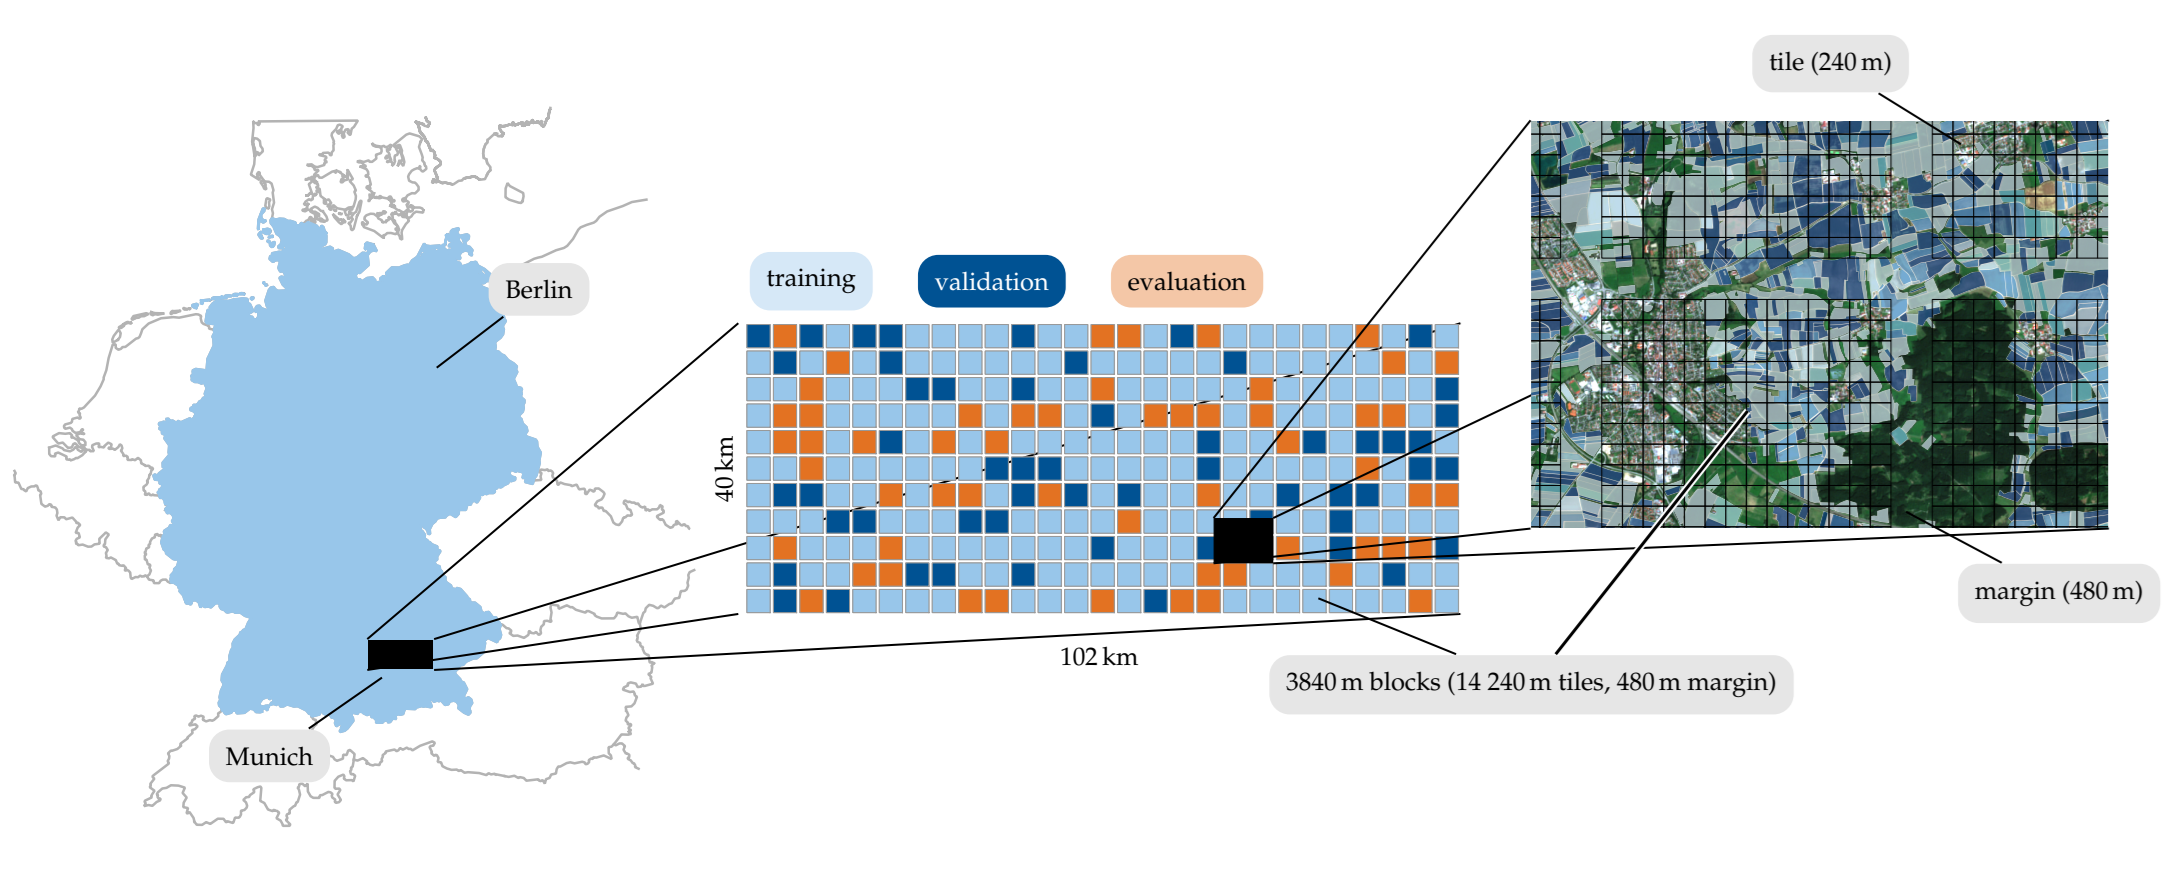
\includegraphics[width=1.0\textwidth]{Immagini/sperimentazione/Munich.png}
        \caption{Rappresentazione dell'area di interesse.}
        \label{fig:MUNICH}
    \end{figure} 
\end{center}


\newpage
\subsection{Lettura dei dati dal dataset}
I dati all'interno del dataset sono organizzati nel seguente modo:
\begin{verbatim}
Munich480/
  data16/                // immagini dell'anno 2016
    1/                    // ID 
      20160103_10m.tif     // acquisizione del 2016-01-03 con tutte le bande da 10m
      20160103_20m.tif     // acquisizione del 2016-01-03 con tutte le bande da 20m
      20160103_60m.tif     // acquisizione del 2016-01-03 con tutte le bande da 60m
      ...
      20161118_10m.tif     // acquisizione del 2016-11-18 con tutte le bande da 10m
      20161118_20m.tif     // acquisizione del 2016-11-18 con tutte le bande da 20m
      20161118_60m.tif     // acquisizione del 2016-11-18 con tutte le bande da 60m            
      y.tif                // mappa di verità della sequenza
    ... 
    14300/             
      20160103_10m.tif
      20160103_20m.tif
      20160103_60m.tif 
      ...
      20161118_10m.tif 
      20161118_20m.tif 
      20161118_60m.tif               
      y.tif
  data17/                // immagini dell'anno 2017
    1/                    // ID 
      20160105_10m.tif     // acquisizione del 2016-01-05 con tutte le bande da 10m
      20160105_20m.tif     // acquisizione del 2016-01-05 con tutte le bande da 20m
      20160105_60m.tif     // acquisizione del 2016-01-05 con tutte le bande da 60m
      ...
    ...
  classes.txt            // File con le informazioni sulle classi
  tileids/                // Informazioni sui tile
    eval.tileids           // File con gli ID da utilizzare per la validazione
    test_fold0.tileids     // File con gli ID da utilizzare per la valutazione
    train_fold0.tileids    // File con gli ID da utilizzare per l'addestramento
\end{verbatim}

Il file \texttt{classes.txt} contiene le informazioni delle classi che sono presenti 
nel dataset.
\begin{verbatim}
    0|unknown           //sconosciuto
    1|sugar beet        //barbabietola da zucchero
    2|summer oat        //avena estiva
    3|meadow            //prato
    5|rape              //colza
    8|hop               //luppolo
    9|winter spelt      //farro invernale
    12|winter triticale //triticale invernale
    13|beans            //fagioli
    15|peas             //piselli
    16|potatoe          //patate
    17|soybeans         //soia
    19|asparagus        //asparagi
    22|winter wheat     //grano invernale
    23|winter barley    //orzo invernale
    24|winter rye       //segale invernale
    25|summer barley    //orzo estivo
    26|maize            //mais
\end{verbatim}

Mentre i file \texttt{.tileids} contengono gli ID dei tile che devono essere utilizzati 
per l'addestramento, per la validazione oppure per la valutazione.
Ad esempio il file \texttt{eval.tileids} contiene:
\begin{verbatim}
    169
    170
    171
    172
    173
    174
    256
    ...
\end{verbatim}

Per poter ottenere i dati dal dataset e utilizzarli per l'addestramento 
della rete neurale, dobbiamo definire una classe che estenda 
la classe \textit{Dataset} di PyTorch e ridefinire i metodi 
speciali: \_\_\textit{len}\_\_ e \_\_\textit{getitem}\_\_.
In questo modo, tale classe potrà essere utilizzata dalla 
classe \textit{DataLoader} di PyTorch per prelevare i dati.
Iniziamo definendo il costruttore della classe e le variabili:
\begin{lstlisting}
from torch.utils.data import Dataset
...

class Munich480(Dataset):
    
    _EVAL_TILEIDS = os.path.join("tileids","eval.tileids")
    _TRAIN_TILEIDS = os.path.join("tileids", "train_fold0.tileids")
    _TEST_TILEIDS = os.path.join("tileids", "test_fold0.tileids")
    _FOLDER_2016: str = "data16"
    _FOLDER_2017: str = "data17"
    
    TemporalSize: Final[int] = 32
    ImageChannelsCount: Final[int] = 13
    ImageWidth: Final[int] = 48
    ImageHeight: Final[int] = 48
    ...

    class Year(Flag):
        Y2016 = auto()
        Y2017 = auto()

    class DatasetMode(Enum):
        TRAINING = auto()
        TEST = auto()
        VALIDATION = auto()

    def __init__(self, DatasetPath:str | None, mode: DatasetMode, year:Year, ...):
        super().__init__()
        ...

        #In base a come voglio utilizzare il dataset, leggo la 
        #sequenza corrispondente.

        match mode:
            case Munich480.DatasetMode.TRAINING:
                self._dataSequenze = np.loadtxt(os.path.join(self.DatasetPath, Munich480._TRAIN_TILEIDS), dtype=int)
                
            case Munich480.DatasetMode.TEST:
                self._dataSequenze = np.loadtxt(os.path.join(self.DatasetPath, Munich480._TEST_TILEIDS), dtype=int)
                
            case Munich480.DatasetMode.VALIDATION:
                self._dataSequenze = np.loadtxt(os.path.join(self.DatasetPath, Munich480._EVAL_TILEIDS), dtype=int)
            case _:
                raise Exception(f"Invalid mode {mode}") 
        
    
        temp = {
            Munich480.Year.Y2016 : Munich480._FOLDER_2016,
            Munich480.Year.Y2017 : Munich480._FOLDER_2017
        }
        
        #dizionario per mappare le sequenze di ogni anno
        years_sequenze: Dict[str, any] = dict()
        range = 0
        
        #Verifichiamo l'integrita' di ogni sequenza e la presenza 
        #di tutti i file
        for available_year in Munich480.Year:
            if available_year in year:
                available_folder = os.listdir(os.path.join(self.DatasetPath, temp[available_year]))
                temp_dict: Dict[str, bool] = dict.fromkeys(available_folder, True) 
                tempList: List[str] = list()

                for idx in self._dataSequenze:
                    if temp_dict.get(str(idx)) is not None and os.path.exists(os.path.join(self.DatasetPath, temp[available_year], str(idx), 'y.tif')):
                        tempList.append(os.path.join(self.DatasetPath, temp[available_year], str(idx)))
                
                npList = np.array(tempList, dtype=object)
                
                years_sequenze[temp[available_year]] = {
                    "sequenze" : npList,
                    "range" : (range, range + len(tempList))
                }
                
                range += len(tempList)

            self._yearsSequenze = years_sequenze
    ...
\end{lstlisting}

Definiamo una funzione che mappa un indice (ovvero l'$i$-esimo elemento del dataset) 
al rispettivo anno ed ID, restituendo il percorso della cartella corrispondente.
\begin{lstlisting}
def mapIndex(self, index: int) -> str:
    for year in self._yearsSequenze.keys():
        year_range: Tuple[int, int] = self._yearsSequenze[year]["range"]
        
        if index >= year_range[0] and index < year_range[1]:
            idx = index - year_range[0]
            data_folder_path = self._yearsSequenze[year]["sequenze"][idx]
            
            return data_folder_path#os.path.join(self._folderPath, year, str(data_folder_index))
            
    raise Exception(f"Index {index} not found in any year range")  
\end{lstlisting}

Implementiamo una funzione per leggere un file \texttt{.tif} . 
Per leggere questi file utilizziamo la libreria \textit{rasterio}, la quale fornisce 
già dei metodi per la lettura di questi file.
\begin{lstlisting}
import rasterio
...

def load_dit_file(self, filePath:str, normalize: bool = True) -> Dict[str,any]:
    with rasterio.open(filePath) as src:
        data = src.read().astype(np.float32)
        profile = src.profile
        
    if normalize:
        data = data * 1e-4
    return {"data" : data, "profile" : profile}
\end{lstlisting}
L'oggetto "\textit{profile}" rappresenta tutte le informazioni sull'immagine: numero di canali, 
posizione geografica dell'immagine, ecc. Mentre "\textit{data}" è l'immagine, 
rappresentata come un array numpy.
Successivamente, definiamo una funzione che restituisce i percorsi di tutti i 
file della sequenza che devono essere caricati.
\begin{lstlisting}
def get_dates(self, path: str, sample_number= int | None) -> list[str]:
    files = os.listdir(path)
    dates = list()
    
    for f in files:
        date = f.split("_")[0]
        if len(date) == 8:  # 20160101
            dates.append(date)

    dates = list(set(dates))
    
    if sample_number is None or sample_number < 0:
        return dates
    
    if len(dates) > sample_number:
        dates = random.sample(dates, sample_number)
    elif len(dates) < sample_number:
        while len(dates) < sample_number:
            dates.append(random.choice(dates))

    #restituisce le date disposte in ordine crescente
    return dates.sort()
\end{lstlisting}

Definiamo la funzione che carica tutta la sequenza temprale di un \textit{Tile}.
\begin{lstlisting}
def load_year_sequenze(self, idx: str) -> dict[str, any]:
    sequenzeFolder = self.mapIndex(idx)
    dates = self.get_dates(path=sequenzeFolder, sample_number=Munich480.TemporalSize)
    profile = None
    
    x: torch.Tensor = torch.empty((Munich480.TemporalSize, Munich480.ImageChannelsCount, Munich480.ImageHeight, Munich480.ImageWidth), dtype=torch.float32)
    
    distance_map = {
        Munich480.Distance.m10: "_10m.tif",
        Munich480.Distance.m20: "_20m.tif",
        Munich480.Distance.m60: "_60m.tif"
    }

    # Itera attraverso ogni data per caricare i dati temporali
    for t, date in enumerate(dates):
        current_channel_index = 0 

        
        for distance, suffix in distance_map.items():
            DataDict = self.load_tif_file(os.path.join(sequenzeFolder, f"{date}{suffix}"))
            data = DataDict['data']
            
            if profile is None:
                profile = DataDict["profile"]
            
            tensor = torch.from_numpy(data).unsqueeze(0) 
            
            if distance != Munich480.Distance.m10:
                tensor = F.interpolate(tensor, size=(Munich480.ImageHeight, Munich480.ImageWidth))
            
            num_channels = tensor.size(1)
            
            x[t, current_channel_index:current_channel_index + num_channels, :, :] = tensor.squeeze(0)
            current_channel_index += num_channels

    y = self.load_tif_file(filePath=os.path.join(sequenzeFolder, "y.tif"), normalize = False)["data"]
    
    #(1, 48, 48) -> (48, 48)
    y = np.squeeze(y, axis=0)
    y = torch.from_numpy(y)

    # permute channels with time_series (t x c x h x w) -> (c x t x h x w)
    x = x.permute(1, 0, 2, 3)

    return {"x": x, "y": y, "profile": profile}
\end{lstlisting}
Infine, definiamo la funzione per ottenere l'$i$-esimo elemento del dataset  
e le funzioni \_\_\textit{len}\_\_ e \_\_\textit{getitem}\_\_.
\begin{lstlisting}
def getItem(self, idx: int) -> dict[str, any]:
    assert idx >= 0 and idx < self.__len__(), f"Index {idx} out of range"
    return self.load_year_sequenze(idx)

def __len__(self) -> int:
    if self.DatasetSize is None:
        self.DatasetSize = self.getSize()
    return self.DatasetSize    

def getSize(self) -> int:
    maxValue = 0
    for year in self._yearsSequenze.keys():
        maxValue = max(maxValue, (self._yearsSequenze[year]["range"][1]))
    return maxValue 
       
def __getitem__(self, idx: int) -> any:
    itemDict = self.getItem(idx)
    itemDict = self.apply_transforms(itemDict)
    return  itemDict['x'], itemDict['y'] 

\end{lstlisting}

La classe così creata verrà instanziata per i vari casi nel seguente modo:
\begin{lstlisting}
TRAIN_DATASET = Munich480(datasetFolder = datasetFolder, mode= Munich480.DatasetMode.TRAINING, year= Munich480.Year.Y2016 | Munich480.Year.Y2017,...)

VAL_DATASET = Munich480(datasetFolder = datasetFolder, mode= Munich480.DatasetMode.VALIDATION, year= Munich480.Year.Y2016 | Munich480.Year.Y2017,...)

TEST_DATASET = Munich480(datasetFolder = datasetFolder, mode= Munich480.DatasetMode.TEST, year= Munich480.Year.Y2016 | Munich480.Year.Y2017,...)  

\end{lstlisting}

Per quanto riguarda le \textit{transforms}, faremo uso delle seguenti:
\begin{lstlisting}
transforms = transforms.Compose([
    transforms.RandomHorizontalFlip(p=0.5),
    transforms.RandomVerticalFlip(p=0.5)
])
\end{lstlisting}

\subsection{Applicazione dell'UNet}
Una possibile architettura applicabile a questo problema è la U-Net, 
trattata nella sezione \ref{section:U-Net}.
Tuttavia, questa rete è stata pensata per operare su immagini 2D, mentre nel nostro caso 
utilizziamo una sequenza temporale composta da 32 immagini che devono 
essere processate simultaneamente. In altre parole, abbiamo un tensore con shape 
[\text{Batch\_Size, TimeSeq, Channels, Width, Height}], 
ma la rete può solo operare con tensori aventi shape 
[\text{Batch\_Size, Channels, Width, Height}].
Un possibile modo per ovviare a questa limitazione consisterebbe nel  
rappresentare tutta la sequenza come un unica immagine composta 
da $32\text{x}13$ canali. Così facendo, otterremmo un tensore con
shape [Batch\_Size, 416, 48, 48], compatibile con l'input richiesto dalla rete. 

Per far svolgere questa operazione, basterebbe semplicemente modificare la funzione 
\_\_\textit{getitem}\_\_ nel seguente modo:
\begin{lstlisting}
def __getitem__(self, idx: int) -> any:
    itemDict = self.getItem(idx)
    itemDict = self.apply_transforms(itemDict)
    x = itemDict['x']
    x = x.view(-1, Munich480.ImageHeight, Munich480.ImageWidth)
    return  x, itemDict['y'] 
\end{lstlisting}


Come avevamo visto dallo schema di architettura della U-Net (\ref{fig:UNET_ORIGINAL}), 
la rete è composta da diversi blocchi che eseguono una serie di convoluzioni in successione. 
Per semplicità, definiamo una classe 
che modelli questa successione di convoluzioni.

\begin{lstlisting}
class Multiple_Conv2D_Block(nn.Module):
    def __init__(self, num_convs: int, in_channels: int, out_channels: int, kernel_size: int, stride: int, padding: int, bias: bool):
        super().__init__()
        ...
        self.blockComponents = nn.Sequential()
        for _ in range(num_convs):  
            self.blockComponents.append(
                nn.Conv2d(
                    in_channels=in_channels, 
                    out_channels=out_channels, 
                    kernel_size=kernel_size, 
                    stride=stride, 
                    padding=padding, 
                    bias=bias
                )
            )      
            in_channels = out_channels
            self.blockComponents.append(nn.BatchNorm2d(out_channels))
            self.blockComponents.append(nn.ReLU(inplace=False))
                
    def forward(self, x):
        return self.blockComponents(x)
\end{lstlisting}
Per quanto riguarda il modello, lo implementiamo nel seguente modo:

\begin{lstlisting}
class UNET(nn.Module):
    _FEATURES: Final[Tuple[int, int, int, int]] = (64,128,256,512)

    def __init__(self, in_Channels, out_Channels, ...)
        ...
        self._EncoderBlocks = nn.ModuleList()
        self._Bottleneck = nn.ModuleList()
        self._DecoderBlocks = nn.ModuleList()
        self._OutputLayer = nn.Sequential()
        self._DownSampler = nn.MaxPool2d(kernel_size=2, stride=2)
        in_feat = self._in_Channel
        
        for feature in self._features:
            self._EncoderBlocks.append(
                Multiple_Conv2D_Block(
                    num_convs=2,
                    in_channels=in_feat, 
                    out_channels=feature, 
                    kernel_size=(3,3), 
                    stride=(1,1), 
                    padding=(1,1),
                    bias=False
                )
            )
            in_feat = feature
            
        self._Bottleneck.append(
            Multiple_Conv2D_Block(
                num_convs=2,
                in_channels=self._features[-1],
                out_channels=self._features[-1]*2,
                kernel_size=3,
                stride=1,
                padding=1,
                bias=True
            )
        )
        for feature in reversed(self._features):
            self._DecoderBlocks.append(
                nn.ConvTranspose2d(
                    in_channels=feature*2,
                    out_channels=feature,
                    kernel_size=2,
                    stride=2
                )
            )
            self._DecoderBlocks.append(
                Multiple_Conv2D_Block(
                    num_convs=2,
                    in_channels=feature*2,
                    out_channels=feature,
                    kernel_size=3,
                    stride=1,
                    padding=1,
                    bias=False
                )
            )
        self._OutputLayer.append(
            nn.Conv2d(
                in_channels=self._features[0],
                out_channels=self._out_channels,
                kernel_size=1
            )
        )
    def forward(self, x) -> Optional[torch.Tensor]:
        skip_connections = []
        
        for encoder_block in self._EncoderBlocks:
            x = encoder_block(x)
            skip_connections.append(x)
            x = self._DownSampler(x)

        x = self._Bottleneck[0](x)

        #revers della lista 
        skip_connections = skip_connections[::-1]

        for i in range(0, len(self._DecoderBlocks), 2):
        
            #ConvTranspose2d sul risultato precedente
            x = self._DecoderBlocks[i](x)
            
            #Ottengo la copia del tensore
            skip_connection = skip_connections[int(i//2)]
            
            if x.shape != skip_connection.shape:
                x = nn.functional.interpolate(x, size=skip_connection.shape[2:])

            #Concateno i tensori
            concat_skip = torch.cat((skip_connection, x), dim=1)
            
            #Eseguo le due convoluzioni 
            x = self._DecoderBlocks[i+1](concat_skip)
        x = self._OutputLayer(x)
        return x

\end{lstlisting}
Mentre per il resto del codice, utilizziamo le stesse funzioni utilizzate per la precedente 
sperimentazione (trattata nella sezione \ref{setion:PRIMO_CODICE}) .
Eseguendo l'addestramento della rete ed osservando i risultati ottenuti sul dataset di 
validazione all'epoca 28 (\ref{fig:UNET_2D_noWeights_confusionMatrix}), ci si accorge 
di un fatto importante:  la rete fatica a classificare correttamente buona parte delle 
classi, soprattutto le classi 3 e 12.

%Mentre sul altre classi il modello fa ancora molta confusione. 

\begin{figure}[H]
    \centering
    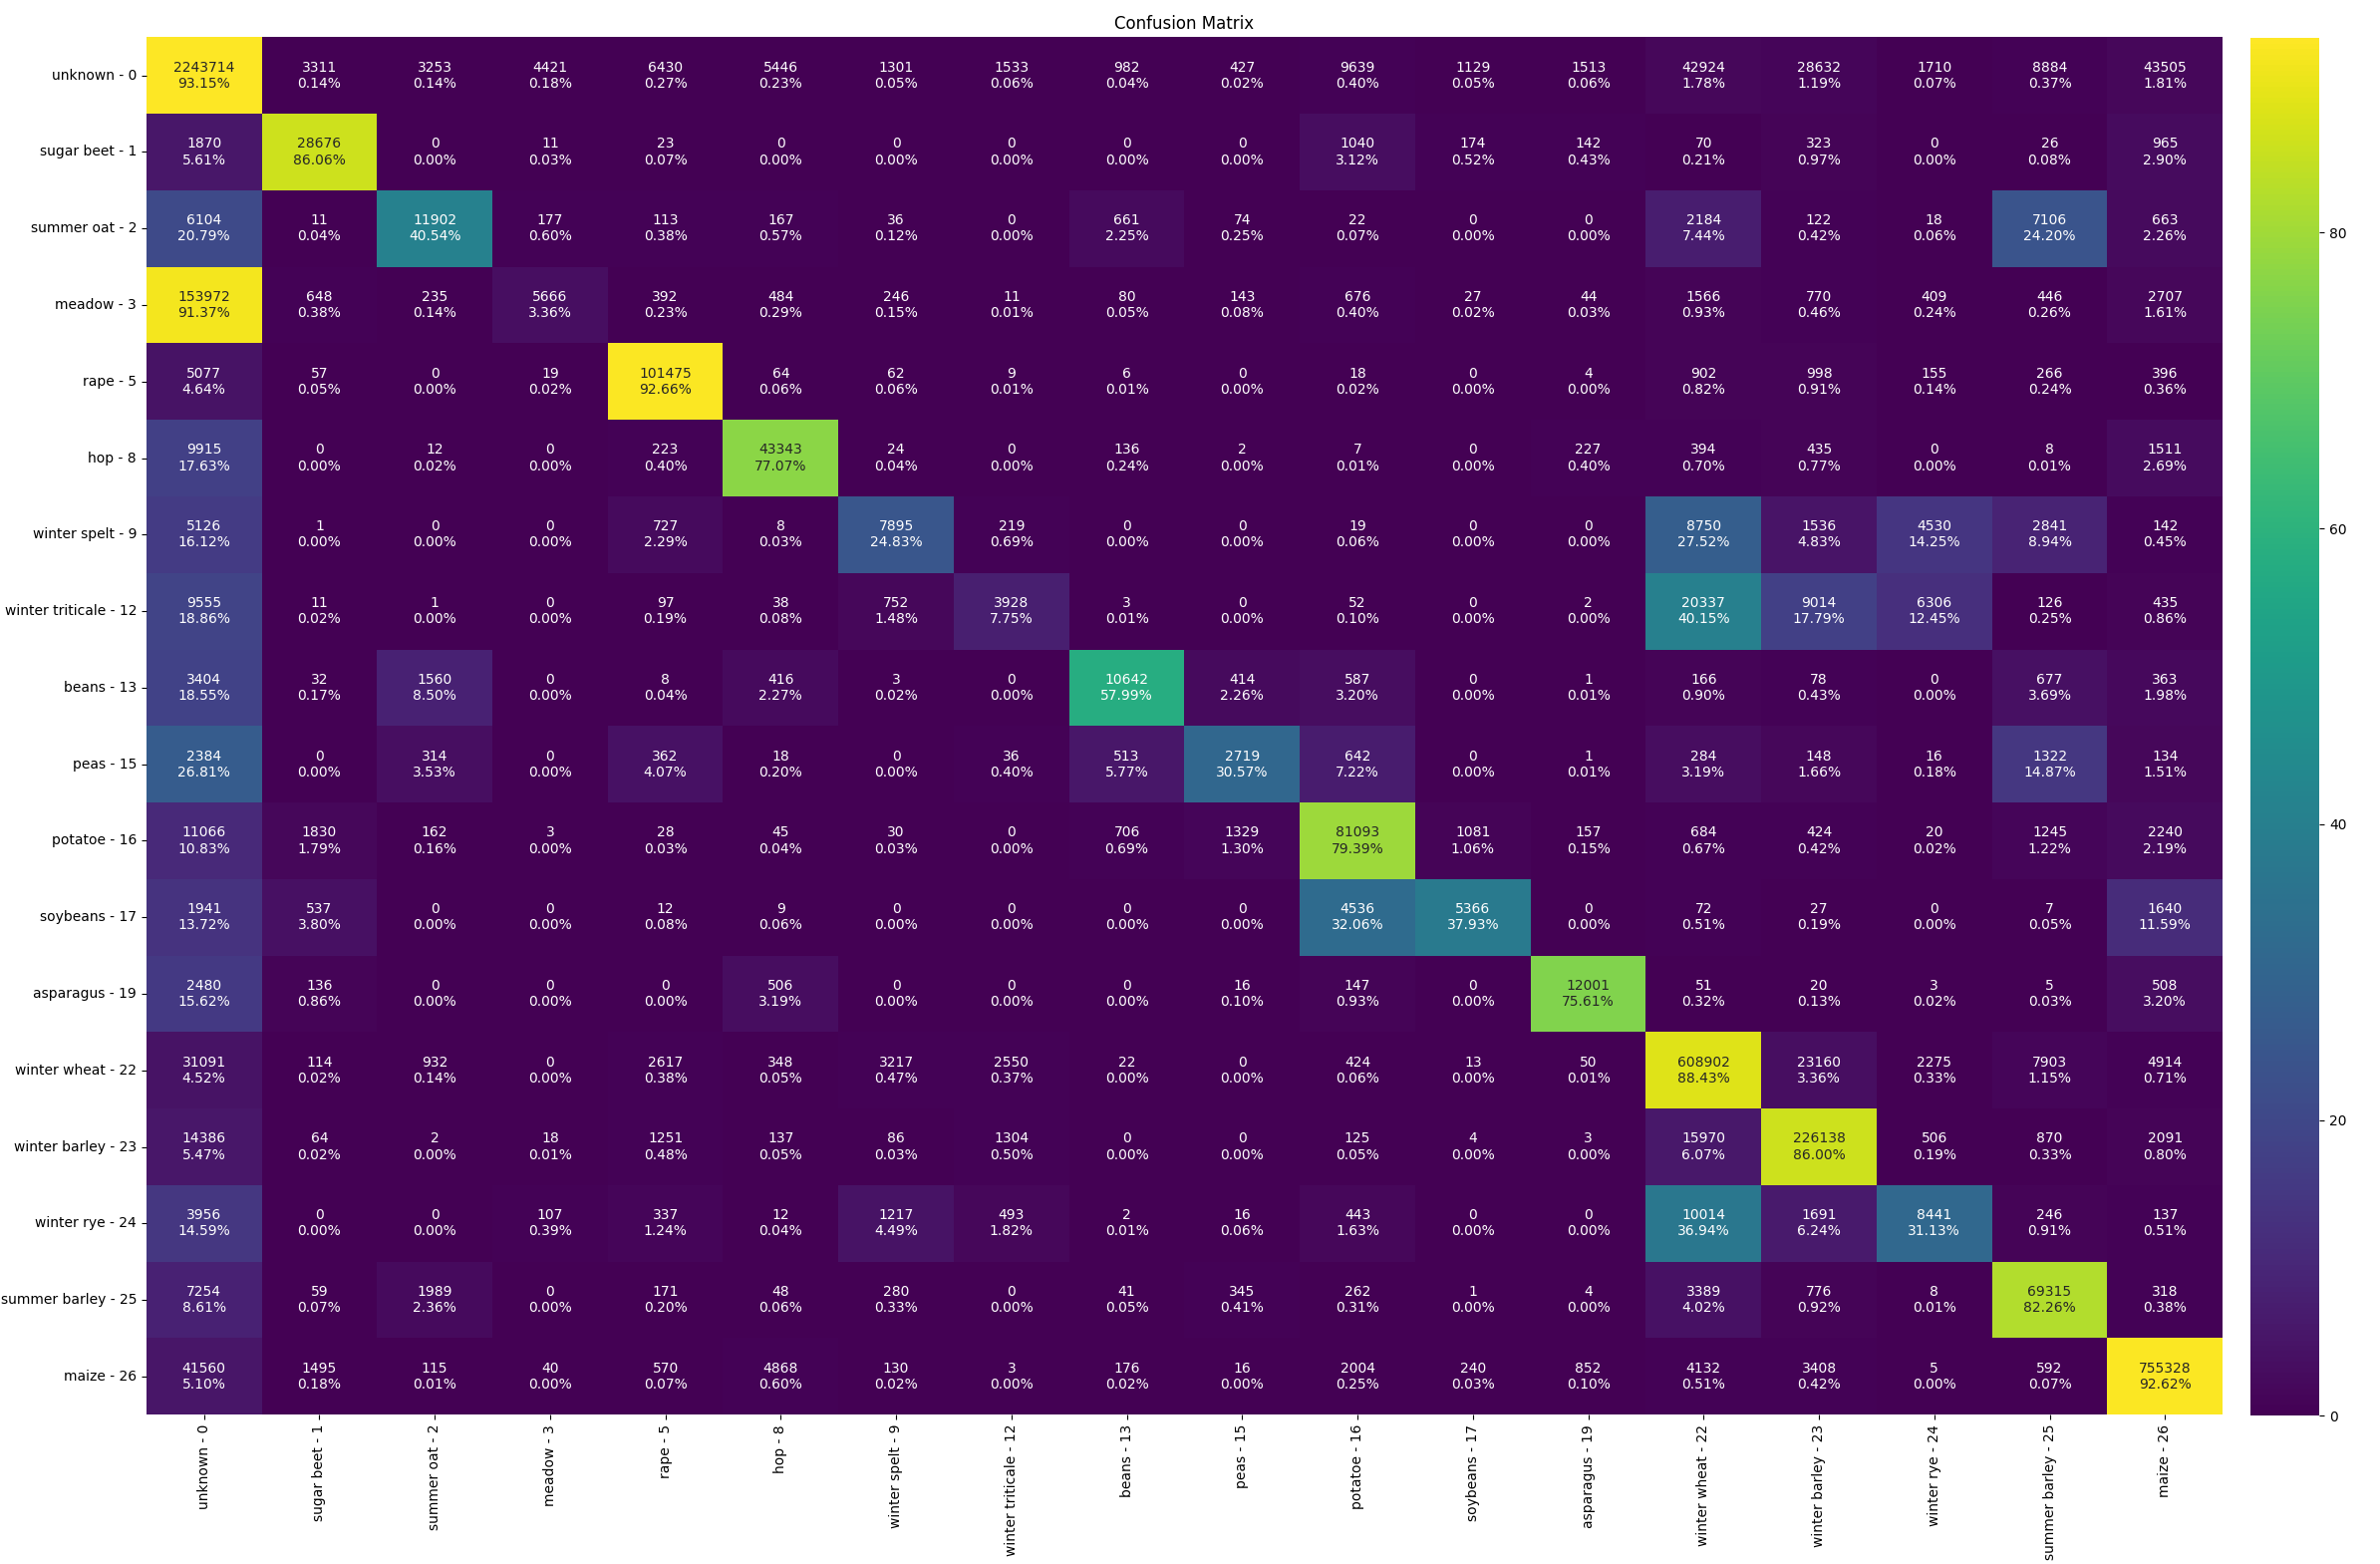
\includegraphics[angle=270,origin=c,width=0.9\textwidth]{Immagini/sperimentazione/UNET_2D_noWeights_confusionMatrix_edit.png}
    \caption{Matrice di confusione del modello.}
    \label{fig:UNET_2D_noWeights_confusionMatrix}

\end{figure} 

Si potrebbe pensare che basterebbe continuare ad addestrare il modello 
ancora per qualche epoca. Tuttavia, osservando  il grafico 
(\ref{fig:UNET_2D_noWeights_accuracy}), possiamo notare come già 
dall'epoca 24 il modello smette di migliorare, mantenendo una precisione poco sotto
all'86\%. Osservando la figura (\ref{fig:UNET_2D_noWeights_confusionMatrix}), si nota che 
questo valore elevato sembra dipendere principalmente dalle classi più numerose.



\begin{figure}[H]
    \centering
    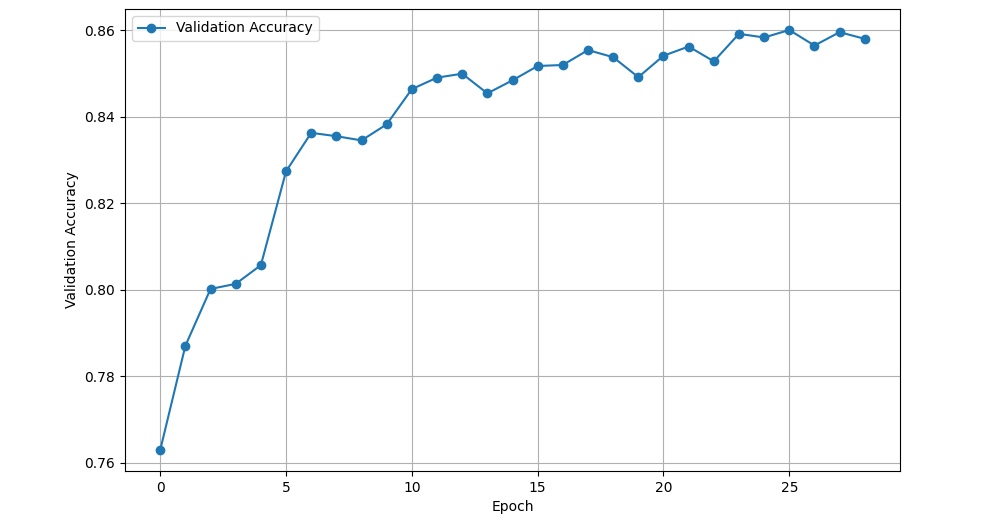
\includegraphics[width=0.96\textwidth]{Immagini/sperimentazione/UNET_2D_noWeights_accuracy.png}
    \caption{Andamento dell'accuratezza.}
    \label{fig:UNET_2D_noWeights_accuracy}
\end{figure}

Analizzando la distribuzione delle classi di verità nelle immagini del 
dataset di training (\ref{fig:Distribuzione_delle_label}), 
possiamo notare come queste classi non siano equilibrate. Di conseguenza, il modello tenderà a 
imparare le classi che si presentano più frequentemente, in quanto 
otterrà una maggiore errore da esse.
Al contrario, per le classi meno frequenti, il modello otterrà un errore 
basso, quasi trascurabile. 
Questo fatto permetterebbe al modello di ottenere un precisione alta solo grazie alle 
classi numerose.
% Ma noi voglio essere in grado di riconoscere quasi perfettamente tutte 
% le classi (o colture).

\begin{figure}[H]
    \centering
    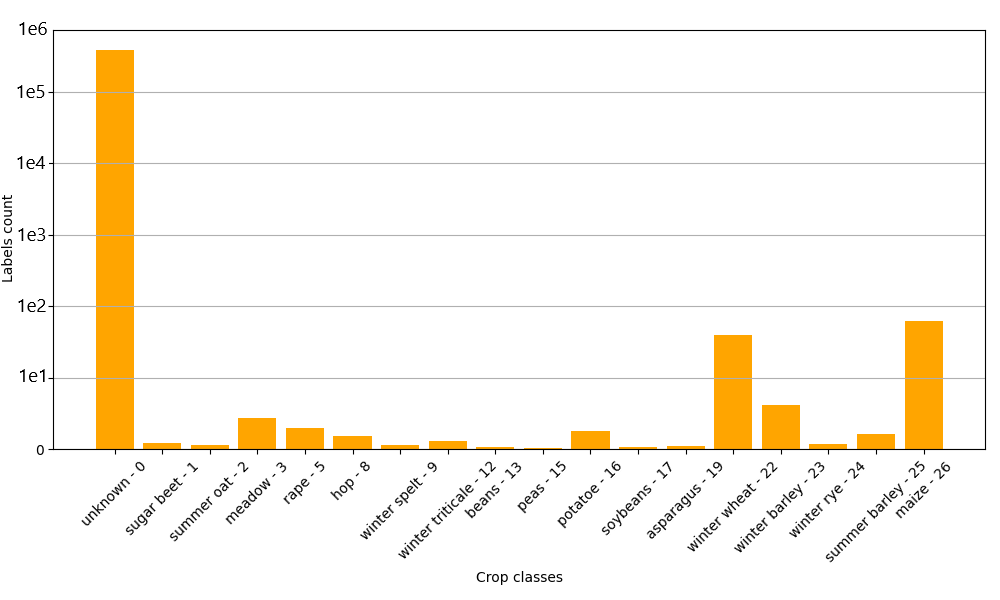
\includegraphics[width=0.80\textwidth]{Immagini/sperimentazione/Distribuzione_delle_label_edited.png}
    \caption{Distribuzione delle classi di verita}
    \label{fig:Distribuzione_delle_label}
\end{figure}

Un modo per risolvere questo problema consisterebbe nell'agire sulla 
funzione di loss, assegnando un peso a ciascuna classe.
Tale peso dipenderebbe dalla frequenza di ciascuna classe e permetterebbe 
di penalizzare fortemente il modello quando sbaglia la predizione 
sulle classi meno frequenti. 

Per il calcolo di questi pesi, ci viene incontro la libreria 
\texttt{sklearn}, in quando offre già delle implementazioni 
da poter utilizzare per il calcolo di questi pesi.

\begin{lstlisting}
from sklearn.utils.class_weight import compute_class_weight 

...

labels, available_classes = count_labels(training_dataset)

class_weights = compute_class_weight(
    class_weight='balanced',
    classes=available_classes,  
    y=labels
)
        
weights = np.zeros(classes_number, dtype=np.float32)
weights[available_classes] = class_weights
weights_tensor = torch.tensor(weights, dtype=torch.float32)

print(weights_tensor)
...

\end{lstlisting}

Una volta eseguiti i calcoli dei pesi, quello che si ottiene è un 
tensore con i seguenti valori:
% \texttt{
% \begin{lstlisting}
% tensor([ 0.1146, 7.2109, 10.3559, 1.4608, 0.0000, 2.1595, 0.0000,  
%     0.0000, 3.5548, 10.7607, 0.0000, 0.0000, 5.4641, 20.7526,  
%     0.0000, 25.7078, 2.5543, 20.7815, 0.0000, 12.0300, 0.0000,  
%     0.0000, 0.4005, 1.0421, 8.3329, 2.9101, 0.3571])
% \end{lstlisting}

\begin{lstlisting}
tensor([ 0.1146, 7.2109, 10.3559, 1.4608, 2.1595,  
    3.5548, 10.7607, 5.4641, 20.7526, 25.7078, 
    2.5543, 20.7815, 12.0300, 0.4005, 1.0421, 
    8.3329, 2.9101, 0.3571])
\end{lstlisting}


% }

Per applicare questi pesi alla funzione di loss basta semplicemente 
scrivere: 
\begin{lstlisting}
lossFunction = nn.CrossEntropyLoss(weight=weights_tensor)
\end{lstlisting}
A questo punto, rieseguiamo il training tenendo conto dei pesi calcolati e vediamo il 
risultato che otteniamo.
\newpage
Dopo aver applicato i pesi ed eseguito il training per 50 epoche, il modello 
raggiunge una precisione massima del 57.60 \%, non riuscendo più a migliorare 
ulteriormente. 

% Questo 
% Applicato  e ripetendo il training, questo è la situazione che 
% abbiamo dopo 50 epoche:
\begin{figure}[H]
    \centering
    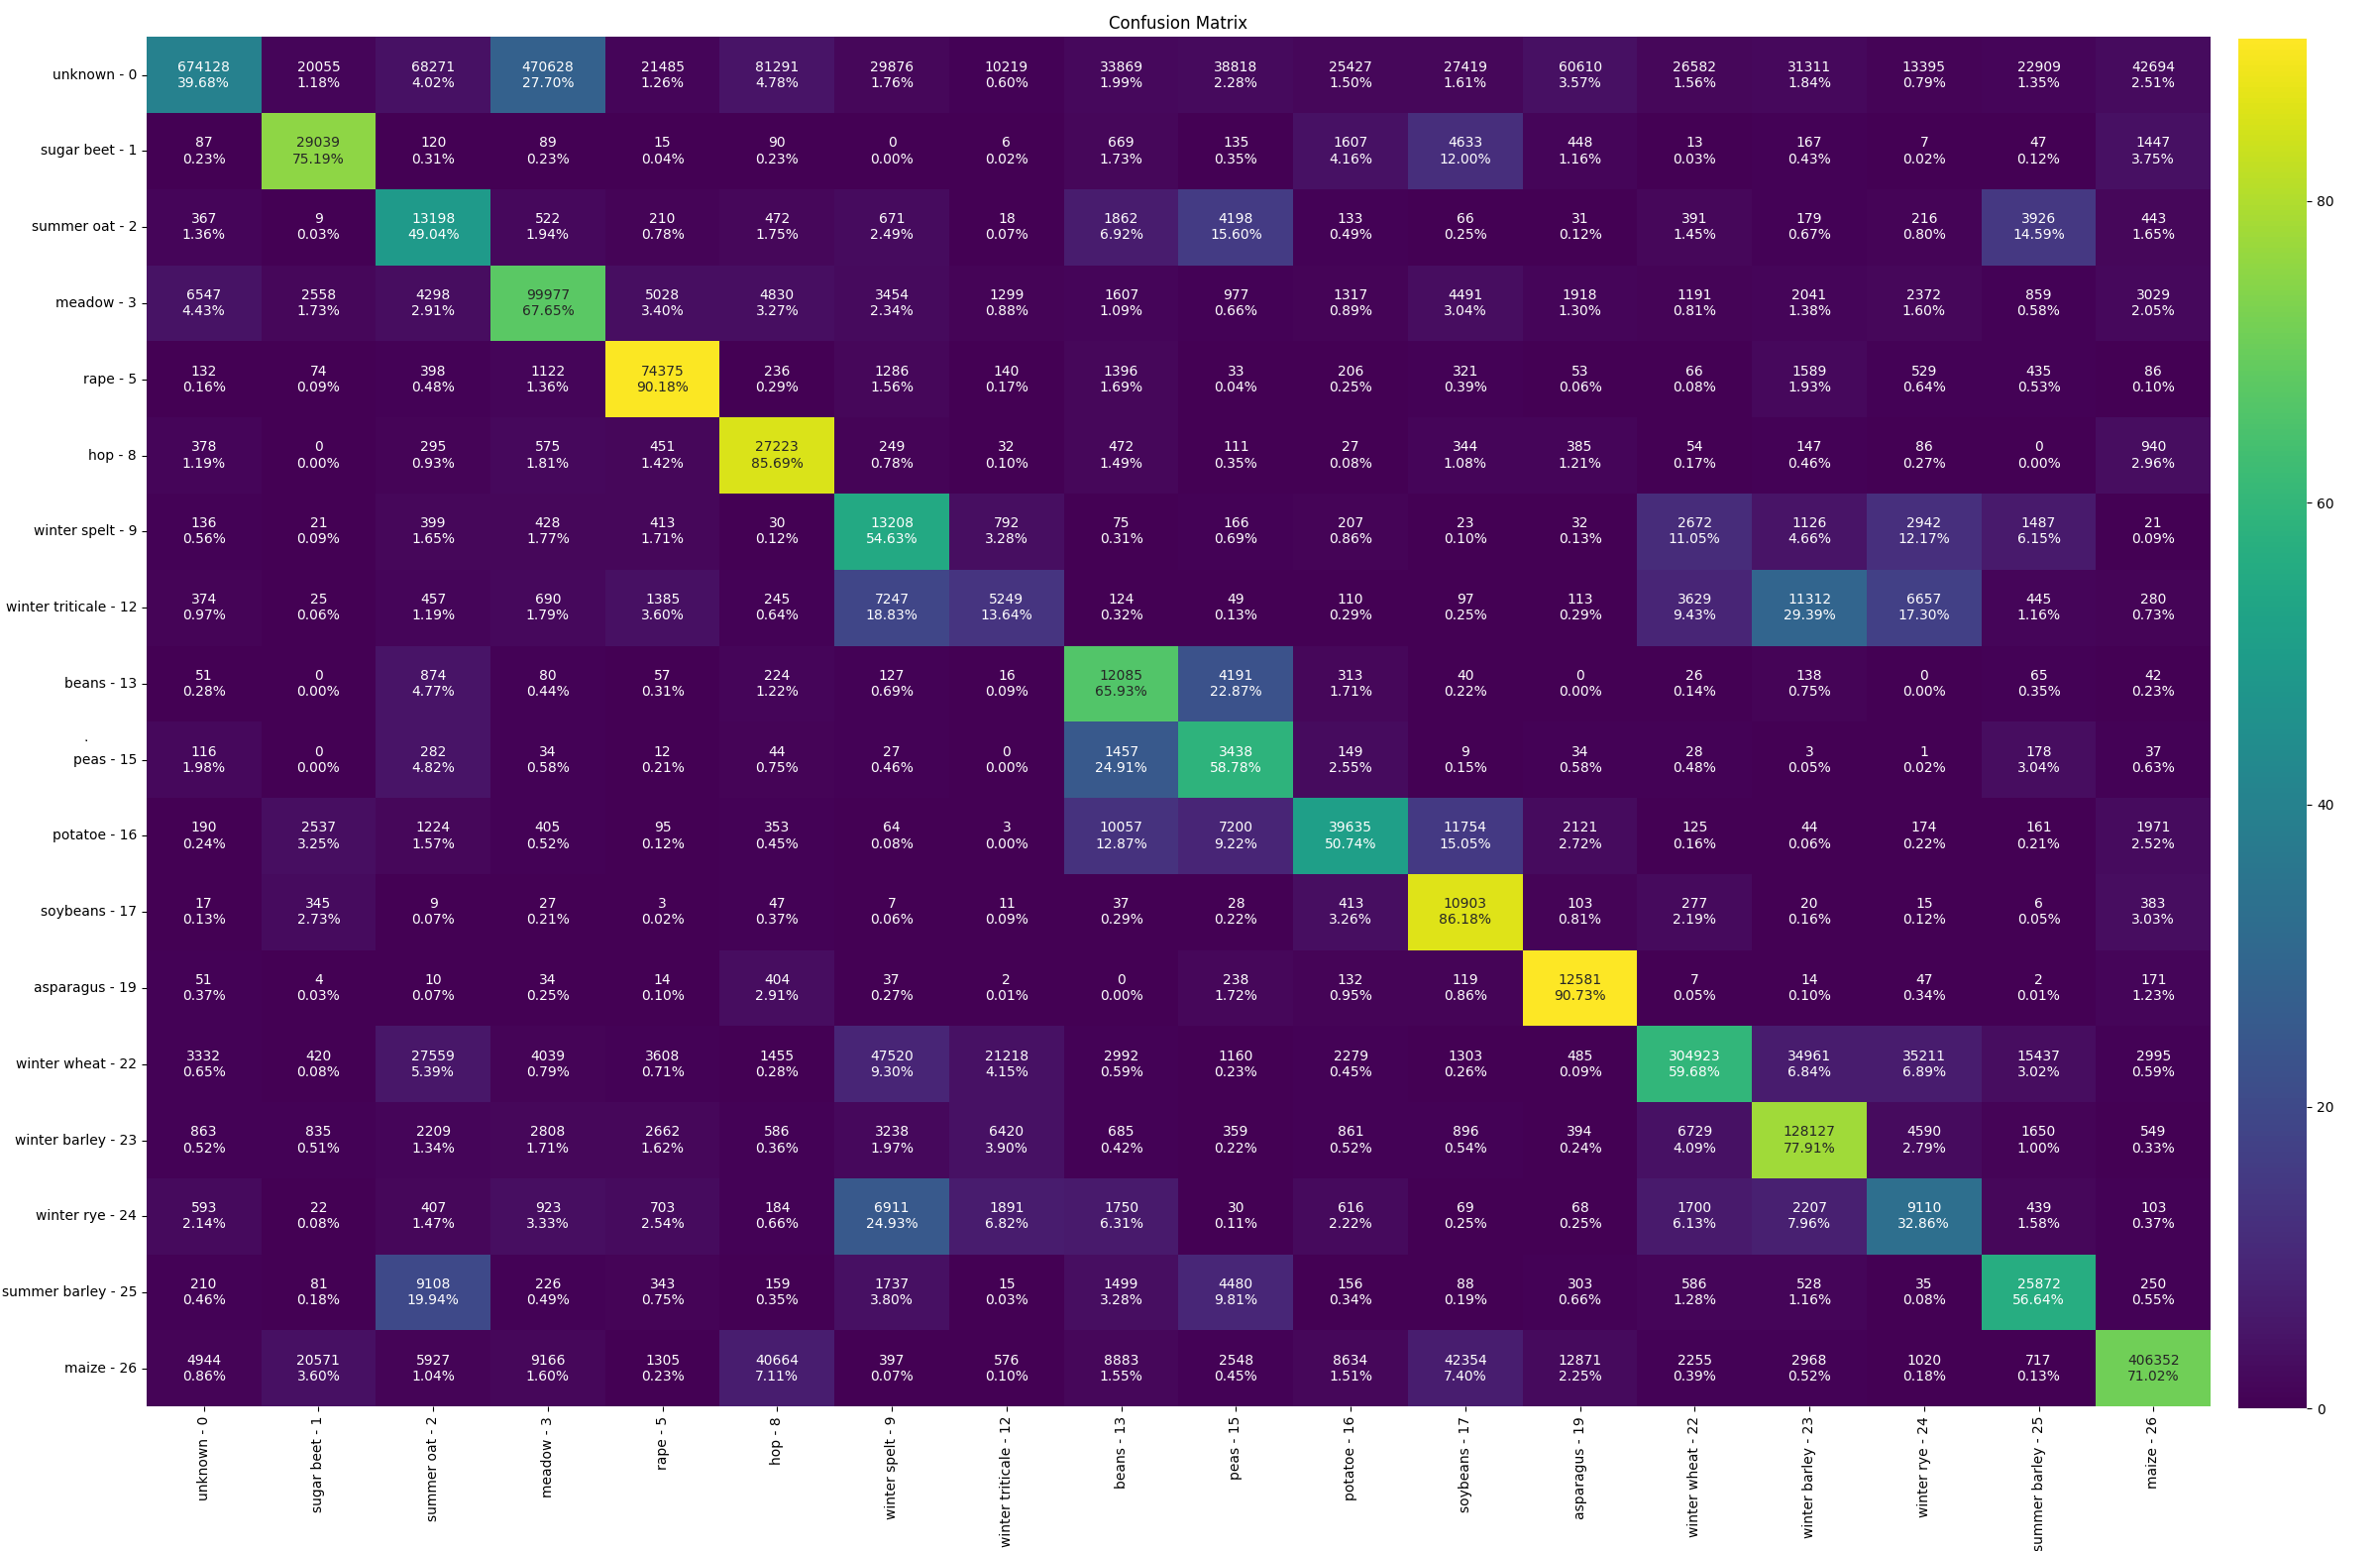
\includegraphics[angle=270,origin=c,width=0.85\textwidth]{Immagini/sperimentazione/UNET_2D_withWeights_confusionMatrix_50_epoche_edit.png}
    \caption{Matrice di confusione del modello dopo avere applicato i pesi.}
    \label{fig:UNET_2D_withWeights_confusionMatrix}
    %Figura 2.1: Esempio schematico di un neurone
\end{figure}

Come possiamo notare dalla matrice di confusione (\ref{fig:UNET_2D_withWeights_confusionMatrix}), 
ora la situazione è bene diversa rispetto a prima 
(\ref{fig:UNET_2D_noWeights_confusionMatrix}). Le classi ora sono più bilanciate, ma 
comunque il modello continua ad avere difficoltà nel distinguere le varie classi, 
soprattutto sulla classe 12. 
Questo sembra essere il massimo ottenibile da questo modello. 
Una possibile soluzione a questo limite potrebbe essere quella di utilizzare una 
versione della U-Net che sfrutti la convoluzione 3D, in modo da poter sfruttare a 
pieno anche le correlazioni temporali tra le immagini.

\subsection{Applicazione della UNet con convoluzioni 3D}
Un modo per superare il limite della UNet con convoluzioni 2D consisterebbe 
nell'utilizzare una sua versione che sfrutta la convoluzione 3D. 
Questa architettura, chiamata anche "3D UNet", 
è tratta in diversi articoli \cite{Articolo1_3D_UNET,Articolo2_3D_UNET} per 
applicazioni con dati volumetrici, come nel nostro caso.
Per implementare questa architetture, ci baseremo su quelle proposte in questi 
repositori \cite{Implementazione1_3D_UNET, Implementazione2_3D_UNET}.
Per implementare questa versione, iniziamo modificando il blocco che 
racchiude le convoluzioni ed adattiamolo per operare in tre dimensioni.

\begin{lstlisting}
class Multiple_Conv3D_Block(nn.Module):
    def __init__(
        self, 
        num_convs: int, 
        in_channels: int, 
        out_channels: int, 
        kernel_size: int | Tuple[int, int, int], 
        stride: int | Tuple[int, int, int] = 1, 
        padding: int | Tuple[int, int, int] = 0, 
        bias: bool = False
    ):
        super(Multiple_Conv3D_Block, self).__init__()
        ...
        self.blockComponents = nn.Sequential()     
        for _ in range(num_convs):  
            self.blockComponents.append(
                nn.Conv3d(
                    in_channels=in_channels, 
                    out_channels=out_channels, 
                    kernel_size=kernel_size, 
                    stride=stride, 
                    padding=padding, 
                    bias=bias
                )
            )
                
        in_channels = out_channels
        self.blockComponents.append(nn.BatchNorm3d(out_channels))
        self.blockComponents.append(nn.ReLU(inplace=True))
        
    def forward(self, x):
        return self.blockComponents(x)
\end{lstlisting}

In questa versione del blocco, è stato introdotto un nuovo elementi, la 
\textit{Batch Normalization} (normalizzazione batch), posto tra ogni convoluzione 
e la usa funzione di attivazione. La \textit{Batch Normalization} permette di 
velocizzare notevolmente il processo di training, mitigando il problema del 
gradiente che svanisce. Consente l'uso di tassi di apprendimento più elevati, 
accelerando la convergenza \cite{Batch_Normalization}.

Modifichiamo anche il blocco che esegue la deconvoluzione definendo una classe 
apposita.
\begin{lstlisting}
    class Deconv3D_Block(nn.Module):
        def __init__(
            self, 
            in_channels: int, 
            out_channels: int, 
            kernel_size: int | Tuple[int, int, int], 
            stride: int | Tuple[int, int, int] = 1, 
            padding: int | Tuple[int, int, int] = 0, 
            bias: bool = False
        ):
        super(Deconv3D_Block, self).__init__()
        ...
        self.deconv = nn.Sequential(
            nn.ConvTranspose3d(
                in_channels, 
                out_channels, 
                kernel_size=kernel_size,
                stride=stride, 
                padding=padding, 
                output_padding=1, 
                bias=bias
            ),
            nn.ReLU(inplace=True)
        )
    def forward(self, x):
        return self.deconv(x)
\end{lstlisting}

Ora passiamo a ridefinire la struttura della rete per adattarla alla versione 3D.
\begin{lstlisting}
class UNet_3D(nn.Module):
    def __init__(self, **kwargs) -> None:
        super(UNet_3D, self)
        ...

        self._DownSampler = nn.MaxPool3d(kernel_size=(2,2,2), stride=(2,2,2))
        in_feat = self._in_Channel
        
        for feature in self._features:
            self._EncoderBlocks.append(
                Multiple_Conv3D_Block(
                    num_convs=2,
                    in_channels=in_feat, 
                    out_channels=feature, 
                    kernel_size=(3,3,3), 
                    stride=(1,1,1), 
                    padding=(1,1,1),
                    bias=True
                )
            )
            in_feat = feature

        self._Bottleneck.append(
            Multiple_Conv3D_Block(
                num_convs=2,
                in_channels=self._features[-1],
                out_channels=self._features[-1]*2,
                kernel_size=3,
                stride=1,
                padding=1,
                bias=True
            )
        )
        for feature in reversed(self._features):
            self._DecoderBlocks.append(
                Deconv3D_Block(
                    in_channels=feature*2,
                    out_channels=feature,
                    kernel_size=(3,3,3),
                    stride=(2,2,2)
                )
            )
            self._DecoderBlocks.append(
                Multiple_Conv3D_Block(
                    num_convs=2,
                    in_channels=feature*2,
                    out_channels=feature,
                    kernel_size=(3,3,3),
                    stride=(1,1,1),
                    padding=(1,1,1),
                    bias=True
                )
            )
        self._OutputLayer = nn.Sequential(
            nn.Conv3d(
                in_channels=self._features[0],
                out_channels=1,
                kernel_size=(1,1,1),
                stride=(1,1,1),
                padding=0,
                bias=True
            ),
            Squeezer(1),
            nn.Conv2d(
                in_channels=self._depth, 
                out_channels=self._out_channels, 
                kernel_size=(1,1), 
                stride=(1,1), 
                padding=0, 
                bias=True
            )
        )
...
\end{lstlisting}
Nello stadio finale della rete, è stato utilizzato un elemento chiamato "\textit{Squeezer}".
Questo elemento è stato creato solo per permettere l'utilizzo dell'operazione di 
\textit{squeeze} all'interno di \textit{nn.Sequential}.
\newpage
Questo elemento "\textit{Squeezer}" è così definito:
\begin{lstlisting}
class Squeezer(nn.Module):
    
    def __init__(self, axes):
        super(Squeezer, self).__init__()
        self.axes = axes
    
    def forward(self, x):
        return x.squeeze(self.axes) 
\end{lstlisting}

Per quanto riguarda la funzione \textit{forward}, essa rimane completamente identica a 
quella utilizzata nella versione 2D.
% Mentre per la funzione \textit{forward}, essa rimane 
% completamente identica a quella utilizzata per la versione 2D.
Passando invece alla classe che gestisce il dataset, riportiamo la funzione 
\_\_\textit{getitem}\_\_  a come era all'inizio, poiché ora 
possiamo operare con tensori 
aventi shape [\textit{Batch\_Size, TimeSeq, Channels, Width}\textit{, Height}].
% Per quanto riguarda la classe che gestisce il dataset, la funzione 
% \_\_\textit{getitem}\_\_ la riportiamo come era all'inizio. 
\begin{lstlisting}
def __getitem__(self, idx: int) -> any:
    itemDict = self.getItem(idx)
    itemDict = self.apply_transforms(itemDict)
    return  itemDict['x'], itemDict['y'] 
\end{lstlisting}
A questo punto, possiamo procedere nuovamente con l'addestramento del modello e vedere i 
risultati che otteniamo. 
\newpage
Dopo aver svolto il training della rete per 70 epoche, la situazione che otteniamo 
è la seguente:

\begin{figure}[H]
    \centering
    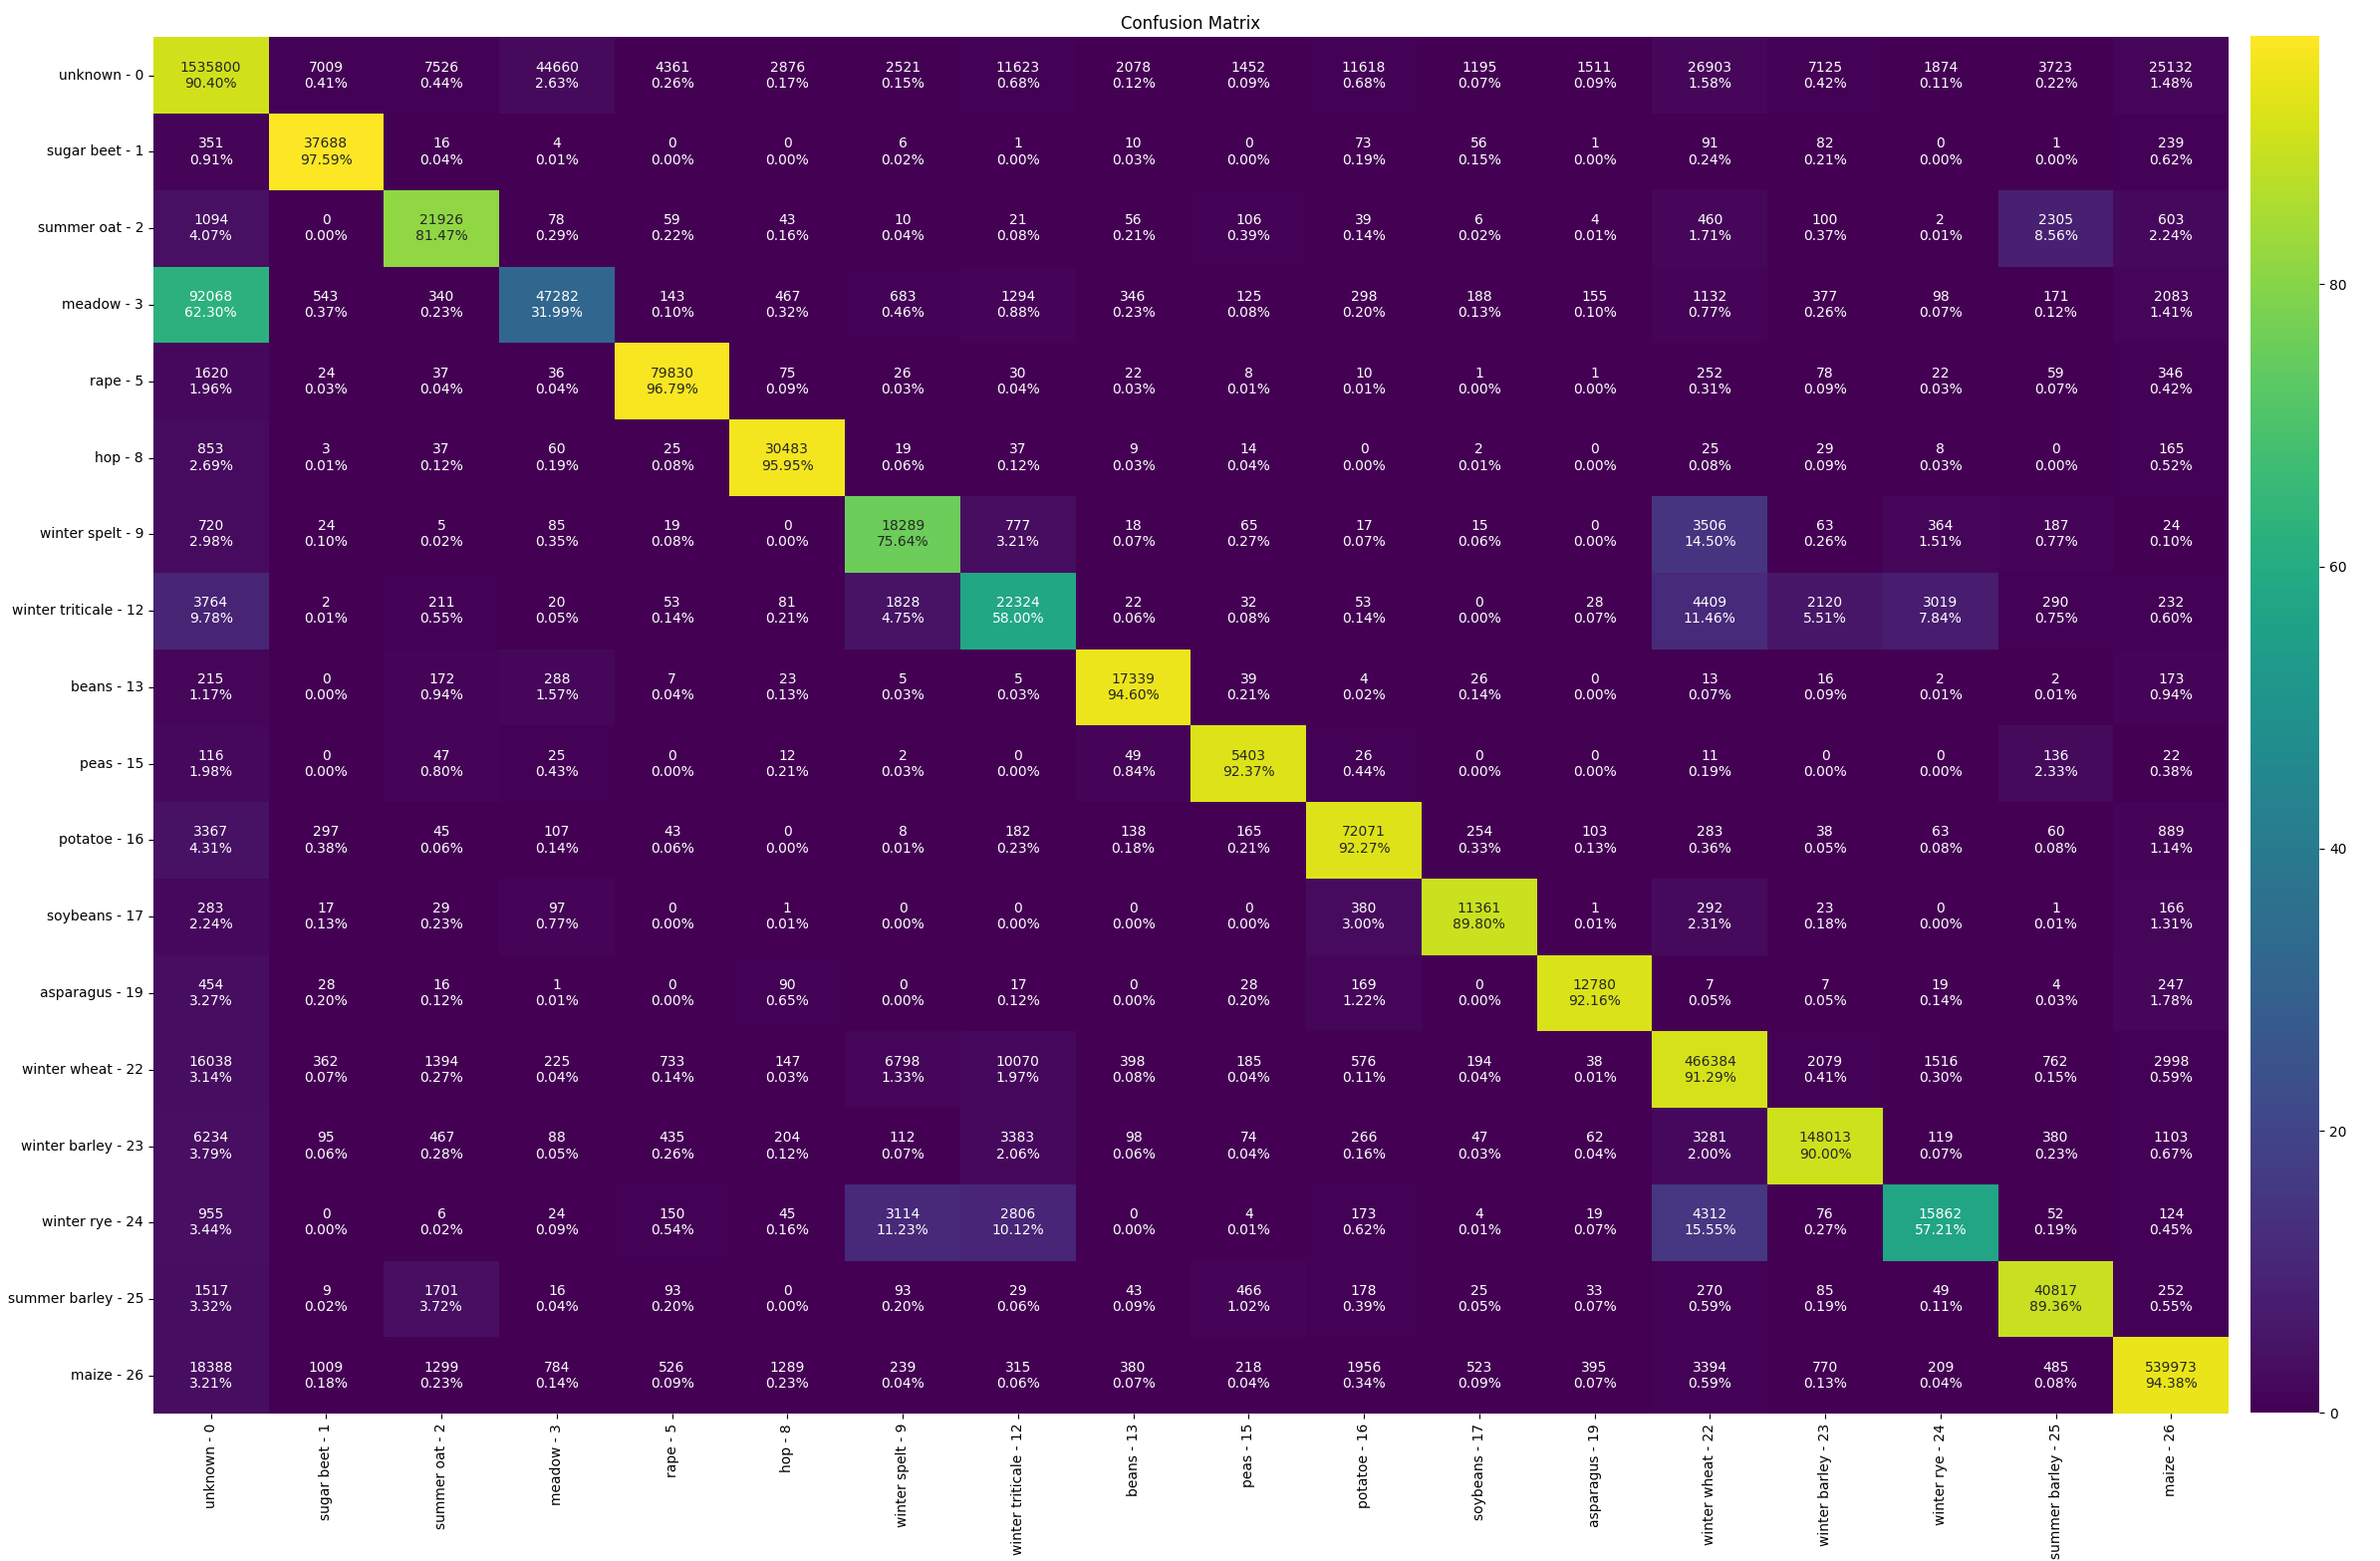
\includegraphics[angle=270,origin=c,width=0.85\textwidth]{Immagini/sperimentazione/UNET_3D_withWeights_confusionMatrix_Edit.png}
    \caption{Matrice di confusione del modello.}
    \label{fig:UNET_3D_withWeights_NoIgnore_confusionMatrix}
    %Figura 2.1: Esempio schematico di un neurone
\end{figure}

Come possiamo osservare dalla figura (\ref{fig:UNET_3D_withWeights_NoIgnore_confusionMatrix}),
la situazione è cambiata notevolmente. Il modello è riuscito ad ottenere dei buoni risultati 
su gran parte delle classi, mostrando una una situazione 
più bilanciata. Tuttavia, il modello fatica ancora a 
classificare correttamente le classi: 3, 12 e 24.
L'utilizzo di questa versione dell'UNet si ha permesso di arrivare ad una  
precisione massima del 88.46\% (\ref{fig:UNET_3D_withWeights_NoIgnore_accuracy}) . 


\begin{figure}[H]
    \centering
    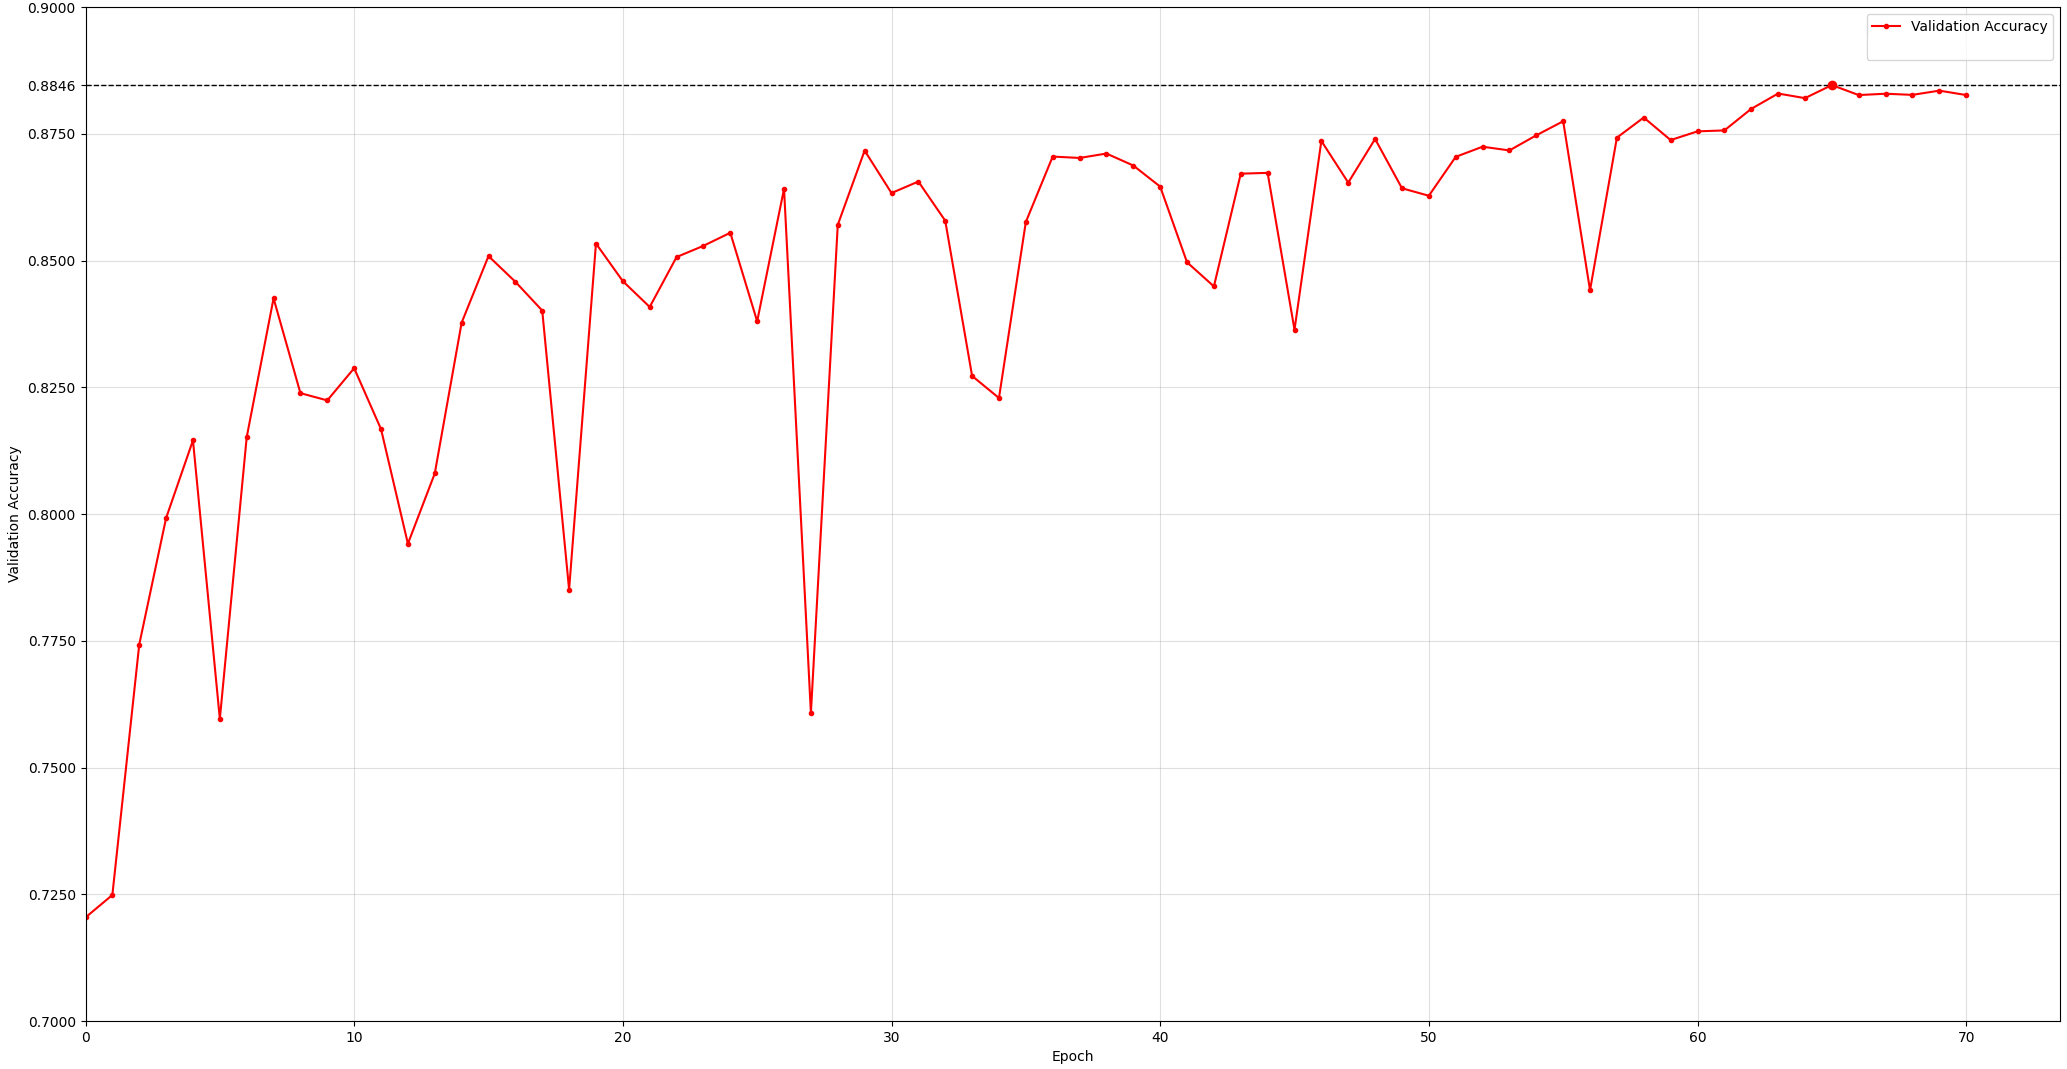
\includegraphics[width=1.02\textwidth]{Immagini/sperimentazione/UNet3D_Weight_noIgnore_accuracy_Edit_v2.png}
    \caption{Andamento dell'accuratezza del modello.}
    \label{fig:UNET_3D_withWeights_NoIgnore_accuracy}
\end{figure}

Proviamo a prendere un campione casuale dal dataset di valutazione e vediamo i risultati 
che otteniamo. La figura (\ref{fig:esempio_immagini_input}) mostra una rappresentazione 
del campione di esempio che viene dato alla rete per svolgere la predizione.

\begin{figure}[H]
    \centering
    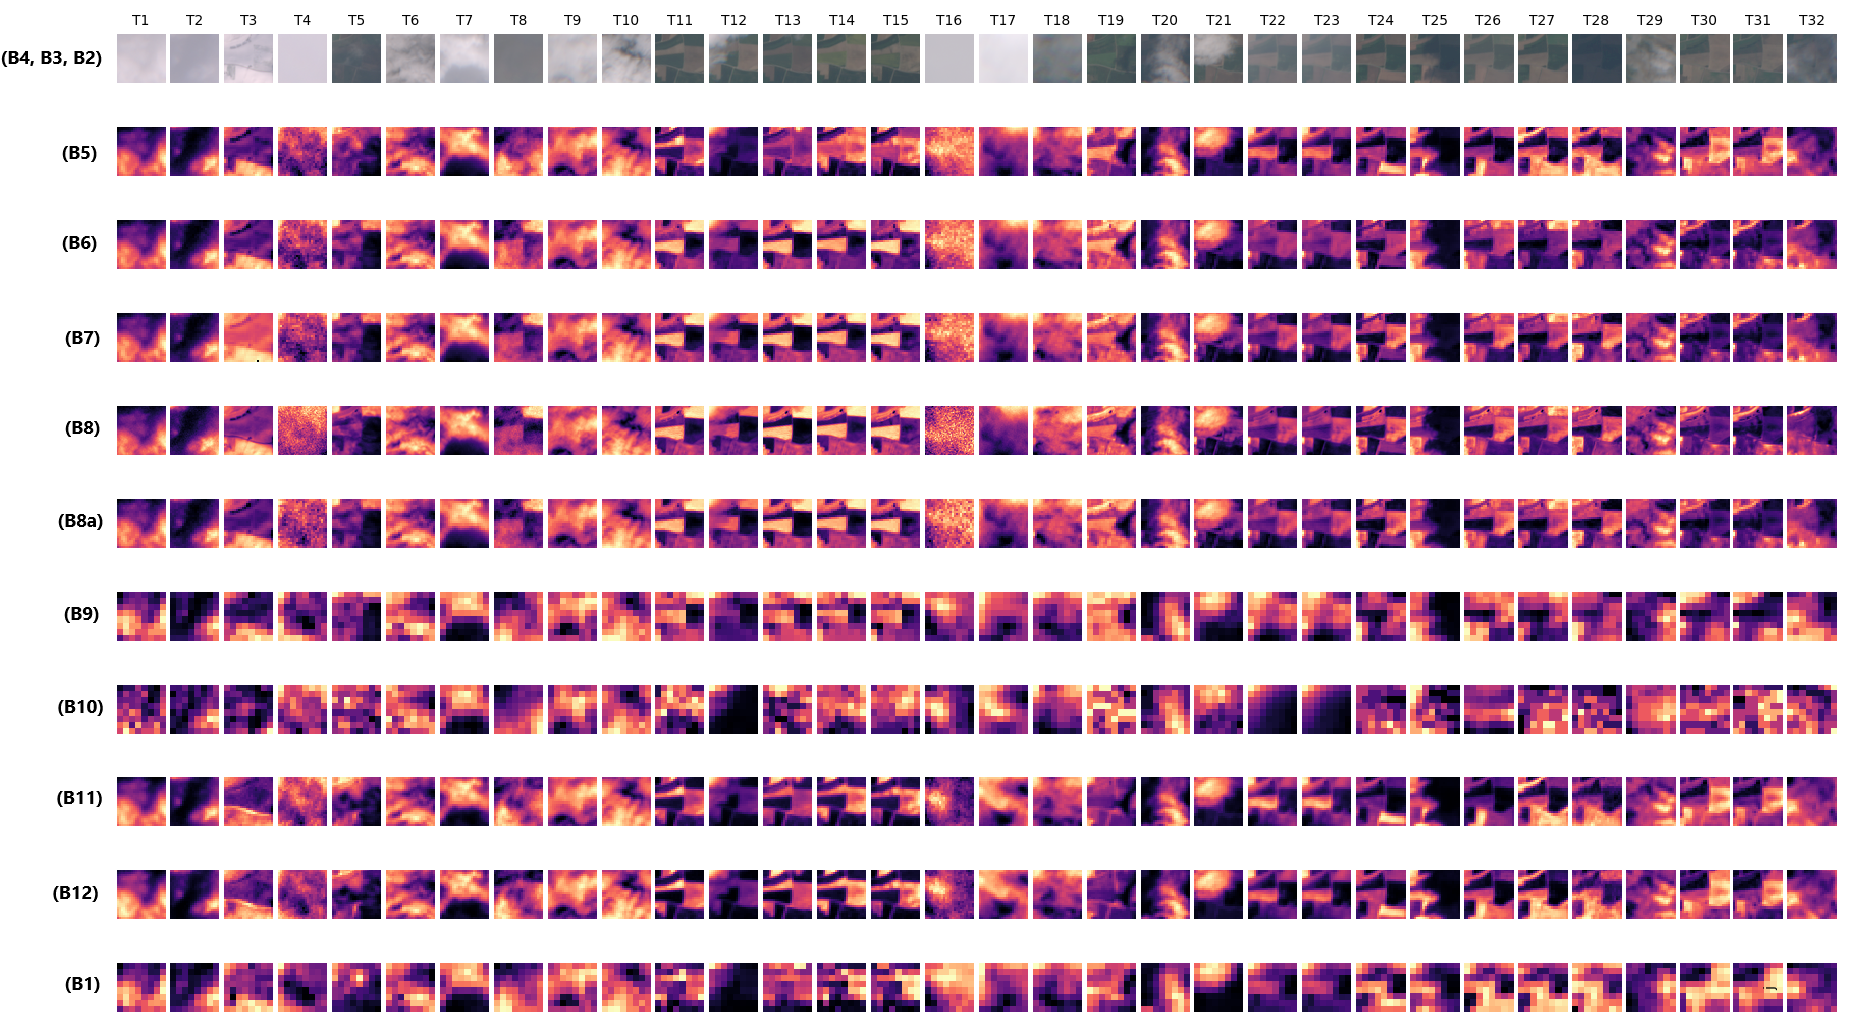
\includegraphics[width=1.05\textwidth]{Immagini/sperimentazione/INPUT_NoIgnore_Edit.png}
    % \caption{Esempio di sequenza temporale fornita alla rete. Le colonne rappresentano le 
    % immagini della sequenza, mentre le righe rappresentano le diverse bande dell'immagine.
    % In alto è riportato il numero della sequenza rappresentato dalla colonna. 
    %A lato sono indicate le bande (o la banda) rappresentate 
    % da ciascuna immagine della riga. 
    % dall'immagine}
    \caption{Esempio di sequenza temporale fornita alla rete. Le colonne rappresentano le 
    immagini della sequenza, mentre le righe corrispondono alle diverse bande. In alto è 
    riportato il numero dell'immagine all'interno della sequenza, mentre a lato sono 
    indicate le bande (o la banda) rappresentate da ciascuna riga.}
    \label{fig:esempio_immagini_input}
\end{figure}

La figura \ref{fig:Esempio_di_output} mostra una rappresentazione dell'output 
ottenuto dalla rete. L'immagine a sinistra è un'immagine casuale scelta dalla 
sequenza \ref{fig:esempio_immagini_input}. L'immagine al centro mostra quello che il 
modello dovrebbe predire, mentre l'immagine a destra mostra il risultato della rete.

\begin{figure}[H]
    \centering
    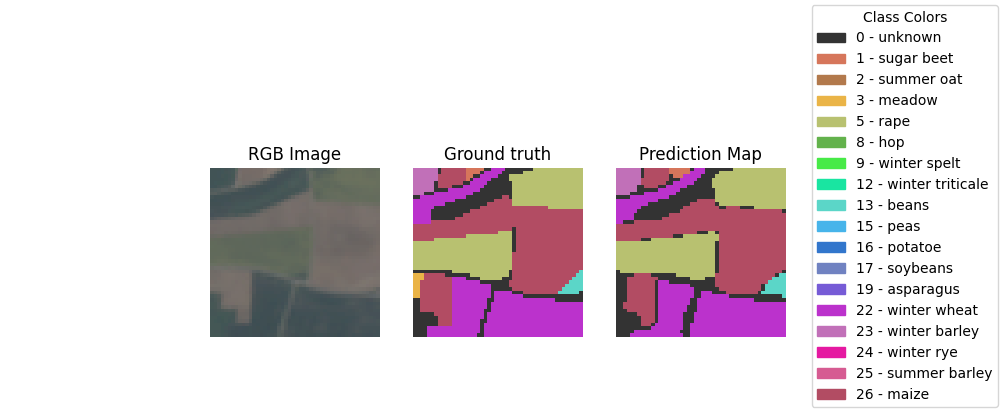
\includegraphics[width=1\textwidth]{Immagini/sperimentazione/LABEL_noIgnore_Edit.png}
    \caption{Rappresentazione dell'input fornito alla rete, del risultato atteso e del risultato ottenuto.}
    \label{fig:Esempio_di_output}
\end{figure}


Come possiamo osservare dalla figura \ref{fig:Esempio_di_output}, il risultato della rete, 
ad eccezione di alcune piccole aree, si è avvicinato molto alla mappa di verità del tile.
Il risultato che abbiamo ottenuto è abbastanza buono, in quanto siamo riusciti a sviluppare un 
modello in grado di riconoscere con precisione questi campi agricoli.
Tuttavia, si potrebbero adottare delle accortezze sulla classe 0 (\textit{unknown}) 
per migliorare ulteriormente la precisione del modello.



\subsection{Ignorare la classe unknown}
Un altro approccio che è possibile utilizzare consiste nell'addestrare la 
rete facendole ignorare la classe "\textit{unknown}", poiché questa classe indica 
solo che non abbiamo informazioni su quello che rappresenta il pixel. Pertanto, potrebbe 
capitare che sia stata assegnata l'etichetta di verità \textit{unknown} ad un pixel che 
potrebbe appartenere a tutt'altra classe, semplicemente perché non si 
era certi dell'effettiva classe di appartenenza del pixel.

Ignorare questa classe \textit{unknown} permetterebbe al modello di concentrarsi solo 
sul riconoscere le classi di cui siamo certi. 
Per implementare questa soluzione, bisognerebbe agire sulla funzione di loss, 
specificandole di escludere la classe 0 (\textit{unknown}) dal calcolo della loss e 
di ignorare le predizioni relative ai pixel la cui etichetta di verità è \textit{unknown}.

Per applicare questa operazione sulla funzione di loss, basta semplicemente fare:
\begin{lstlisting}
lossFunction = nn.CrossEntropyLosss(weight=weights_tensor, ignore_index=0)
\end{lstlisting}

A questo punto rifacciamo di nuovo il training e vediamo i risultati che otteniamo. 
\newpage
Dopo Avere addestrato la rete per 72 epoche, questi sono i risultati che si ottengono:

\begin{figure}[H]
    \centering
    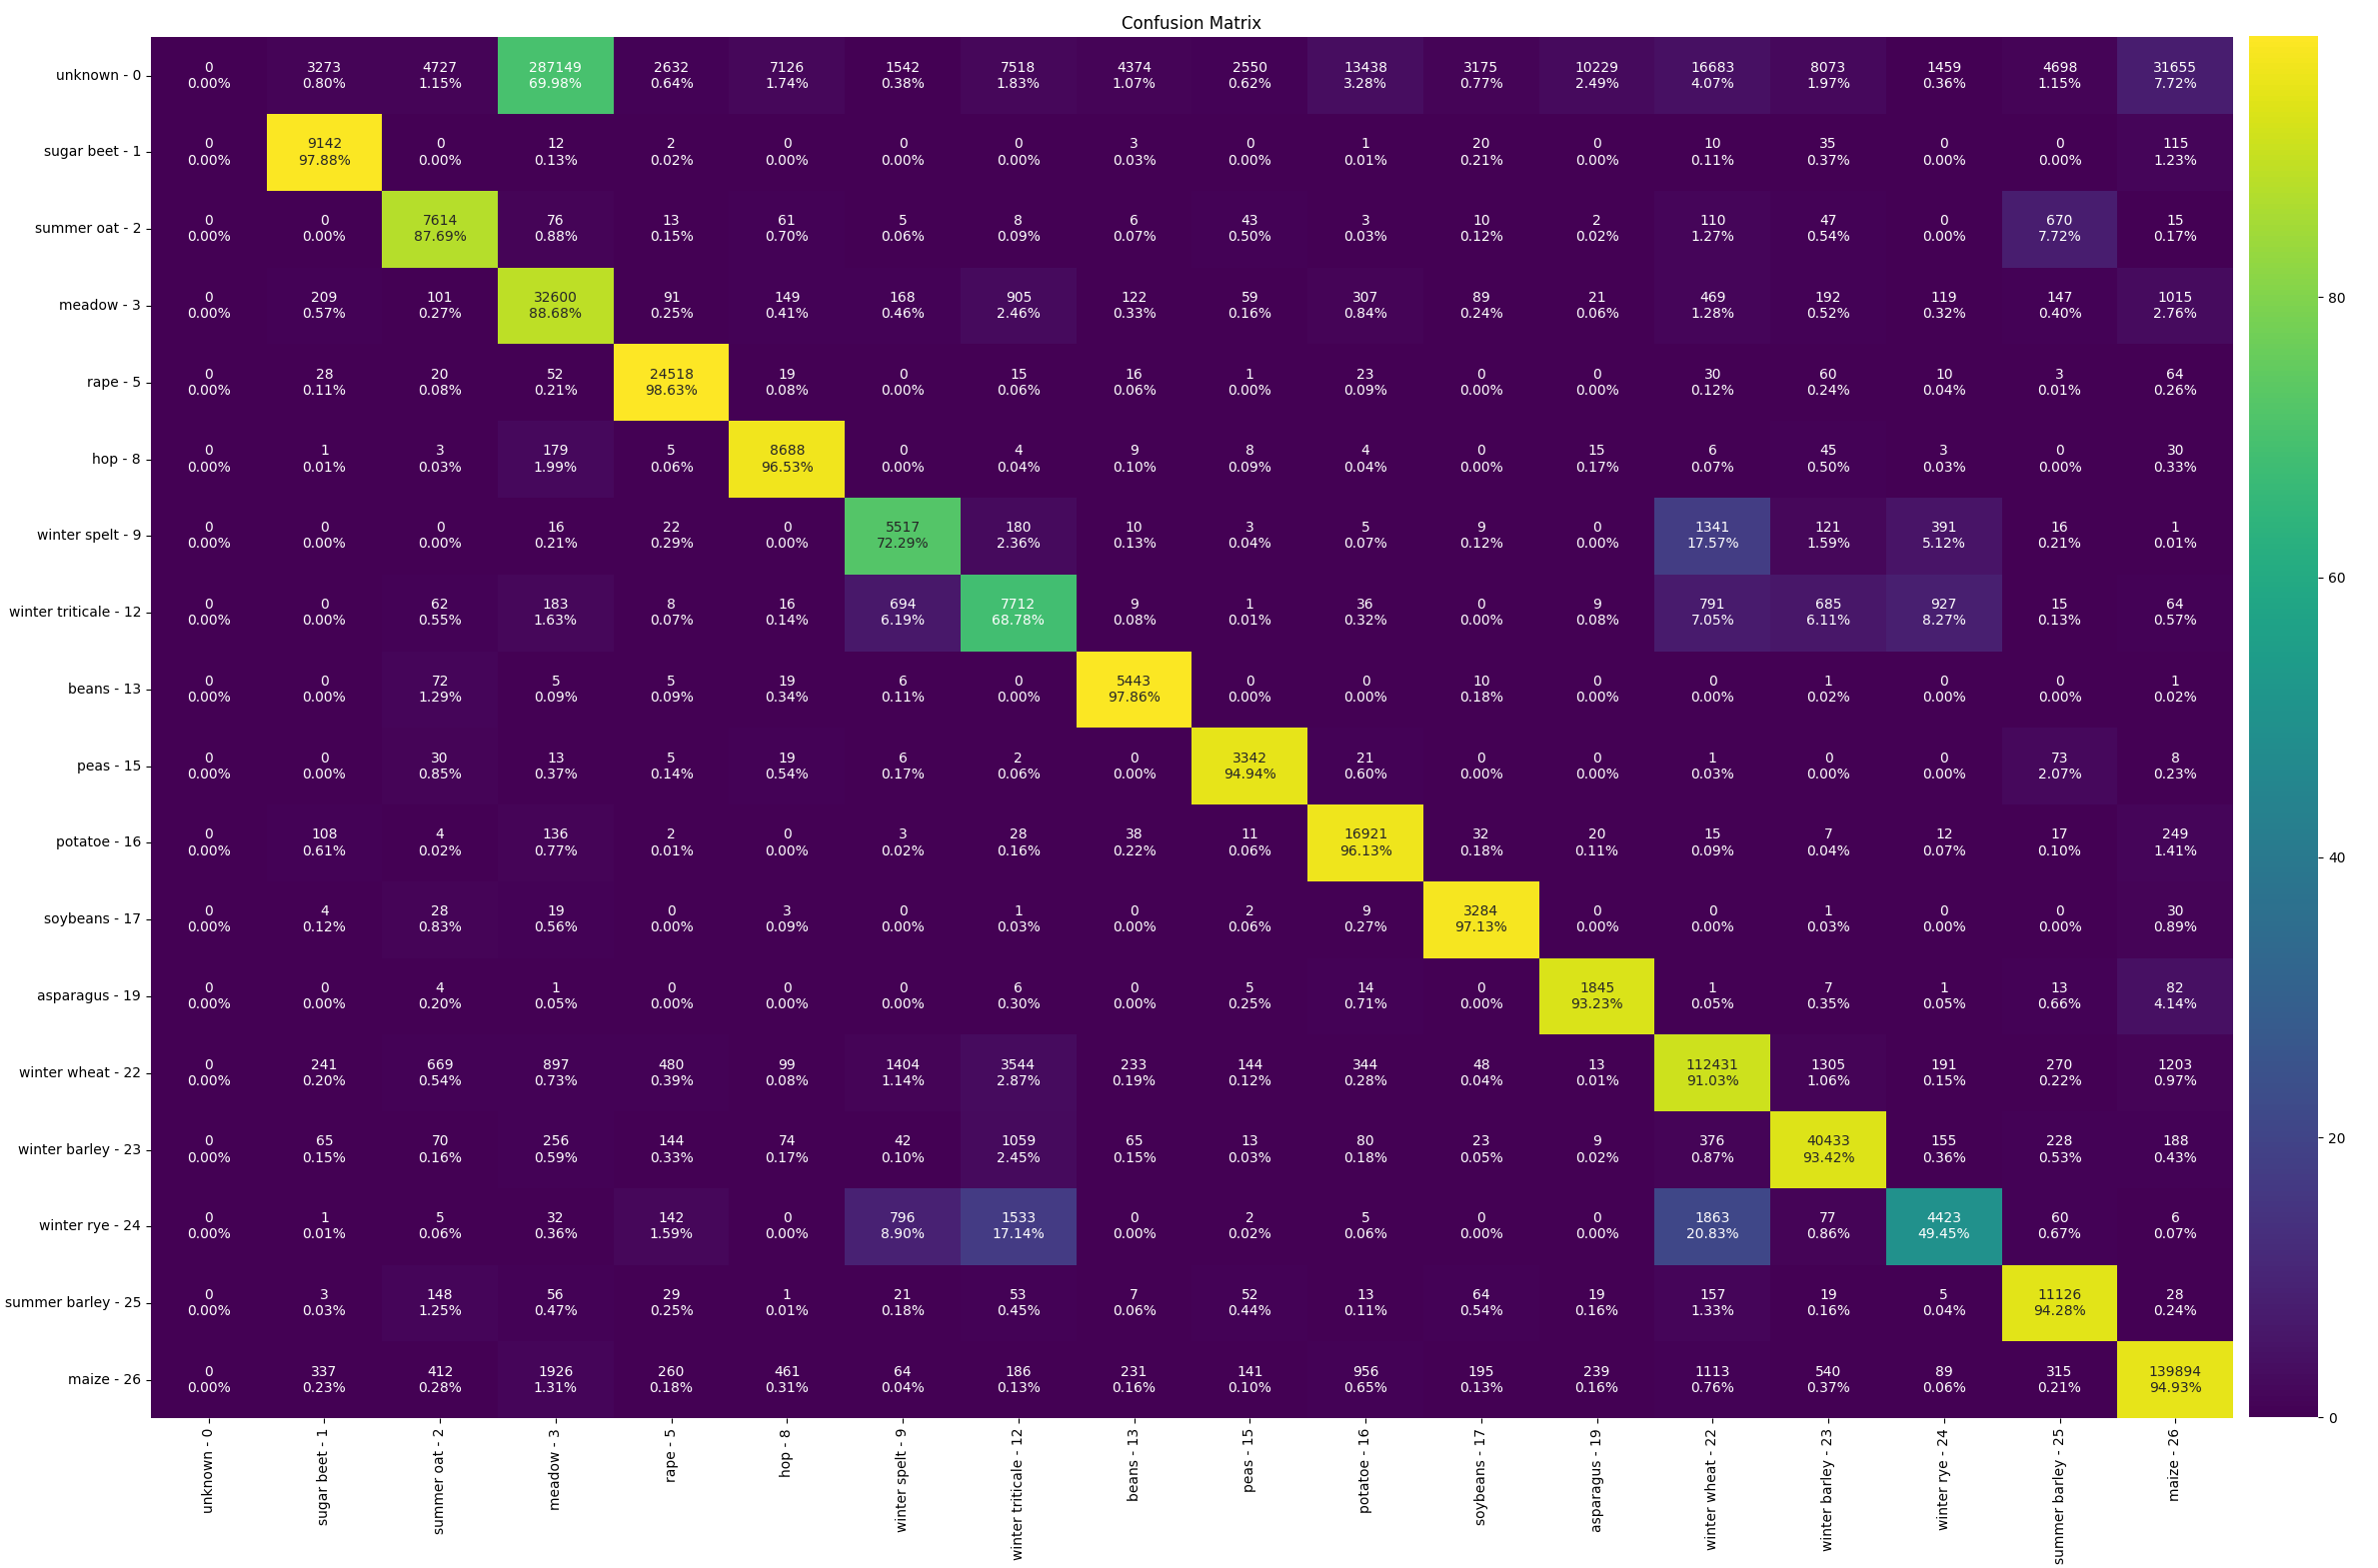
\includegraphics[angle=270,origin=c,width=0.85\textwidth]{Immagini/sperimentazione/UNET_3D_withWeights_Ignore_confusionMatrix_edited.png}
    \caption{Matrice di confusione del modello dopo aver ignorato la classe 0}
    \label{fig:UNET_3D_withWeights_Ignore_confusionMatrix}
\end{figure}

Come possiamo osservare, la situazione è ulteriormente migliorata rispetto a prima 
(\ref{fig:UNET_3D_withWeights_NoIgnore_confusionMatrix}).
Si riscontra ancora una leggera imprecisione sulle classi 24, 12 e 9, dovuta principalmente 
alla loro somiglianza con altre classi. In ogni caso, siamo riusciti a raggiungere una 
precisione (escludendo dal calcolo la classe 0) del 91.8\% 
(\ref{fig:UNET_3D_withWeights_Ignore_accuracy}), limitandoci solo a classificare i 
pixel di cui conosciamo la corretta classe di verità .
%solo svolgendo una classificazione sulle classi dei pixel che sappiamo essere corrette.
Un altro aspetto che si nota dalla figura \ref{fig:UNET_3D_withWeights_Ignore_confusionMatrix} 
è come molti pixel, che erano etichettati come \textit{unknown}, siano 
stati classificati dal modello come appartenenti alla classe 3 (\textit{meadow}).

\begin{figure}[H]
    \centering
    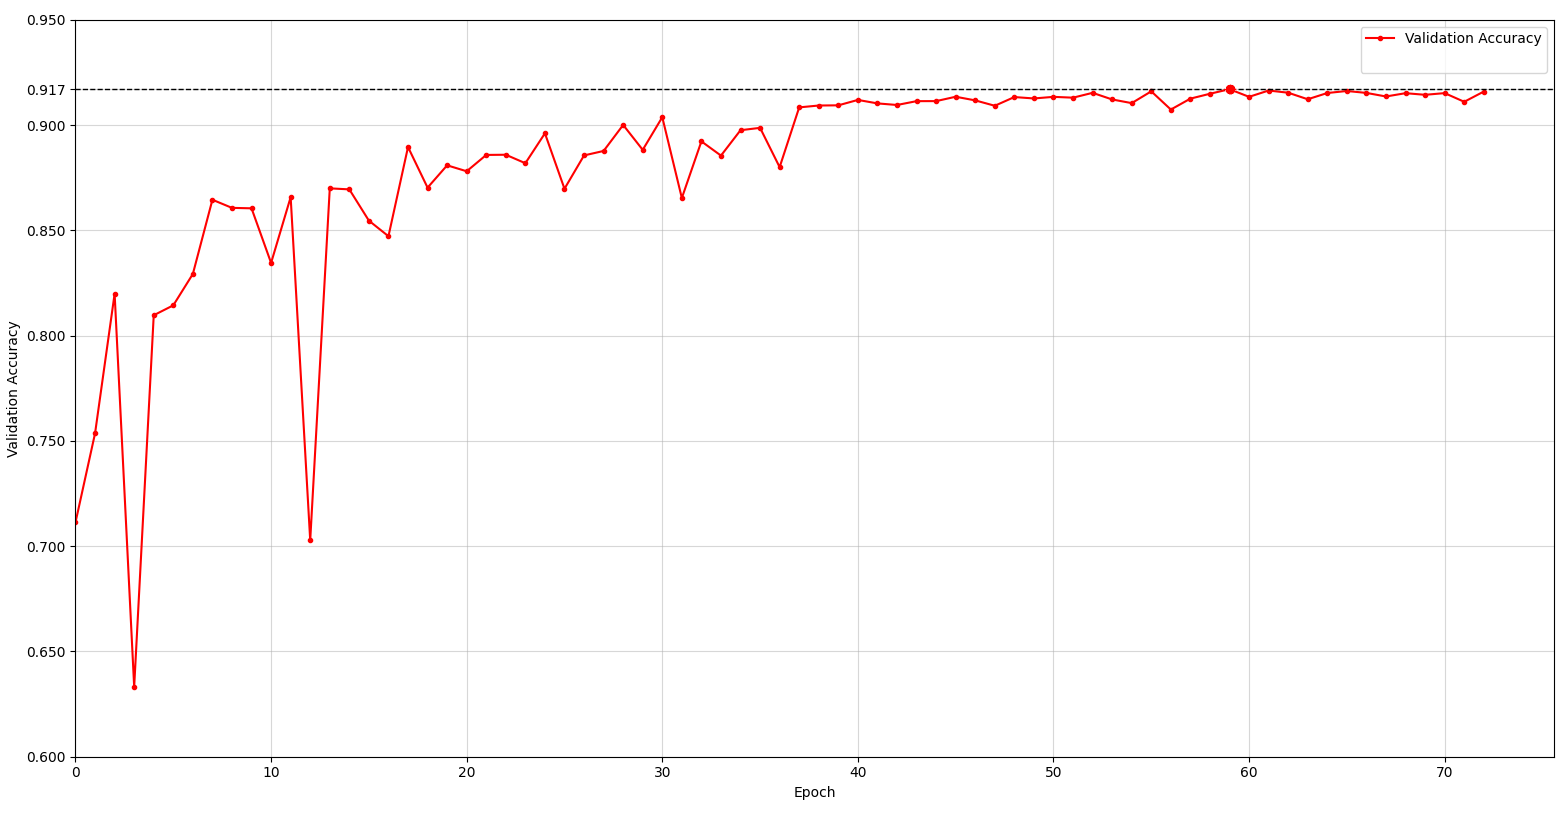
\includegraphics[width=1.02\textwidth]{Immagini/sperimentazione/UNet3D_Weight_Ignore_accuracy_edited_v2.png}
    \caption{Accuratezza del modello.}
    \label{fig:UNET_3D_withWeights_Ignore_accuracy}
\end{figure}


Con questo campione di esempio (\ref{fig:Ignore_INPUT}), possiamo osservare,  
dalle figure \ref{fig:Ignore_LABELS} e \ref{fig:Activations}, come il modello si 
comporta con questo nuovo approccio.
\begin{figure}[H]
    \centering
    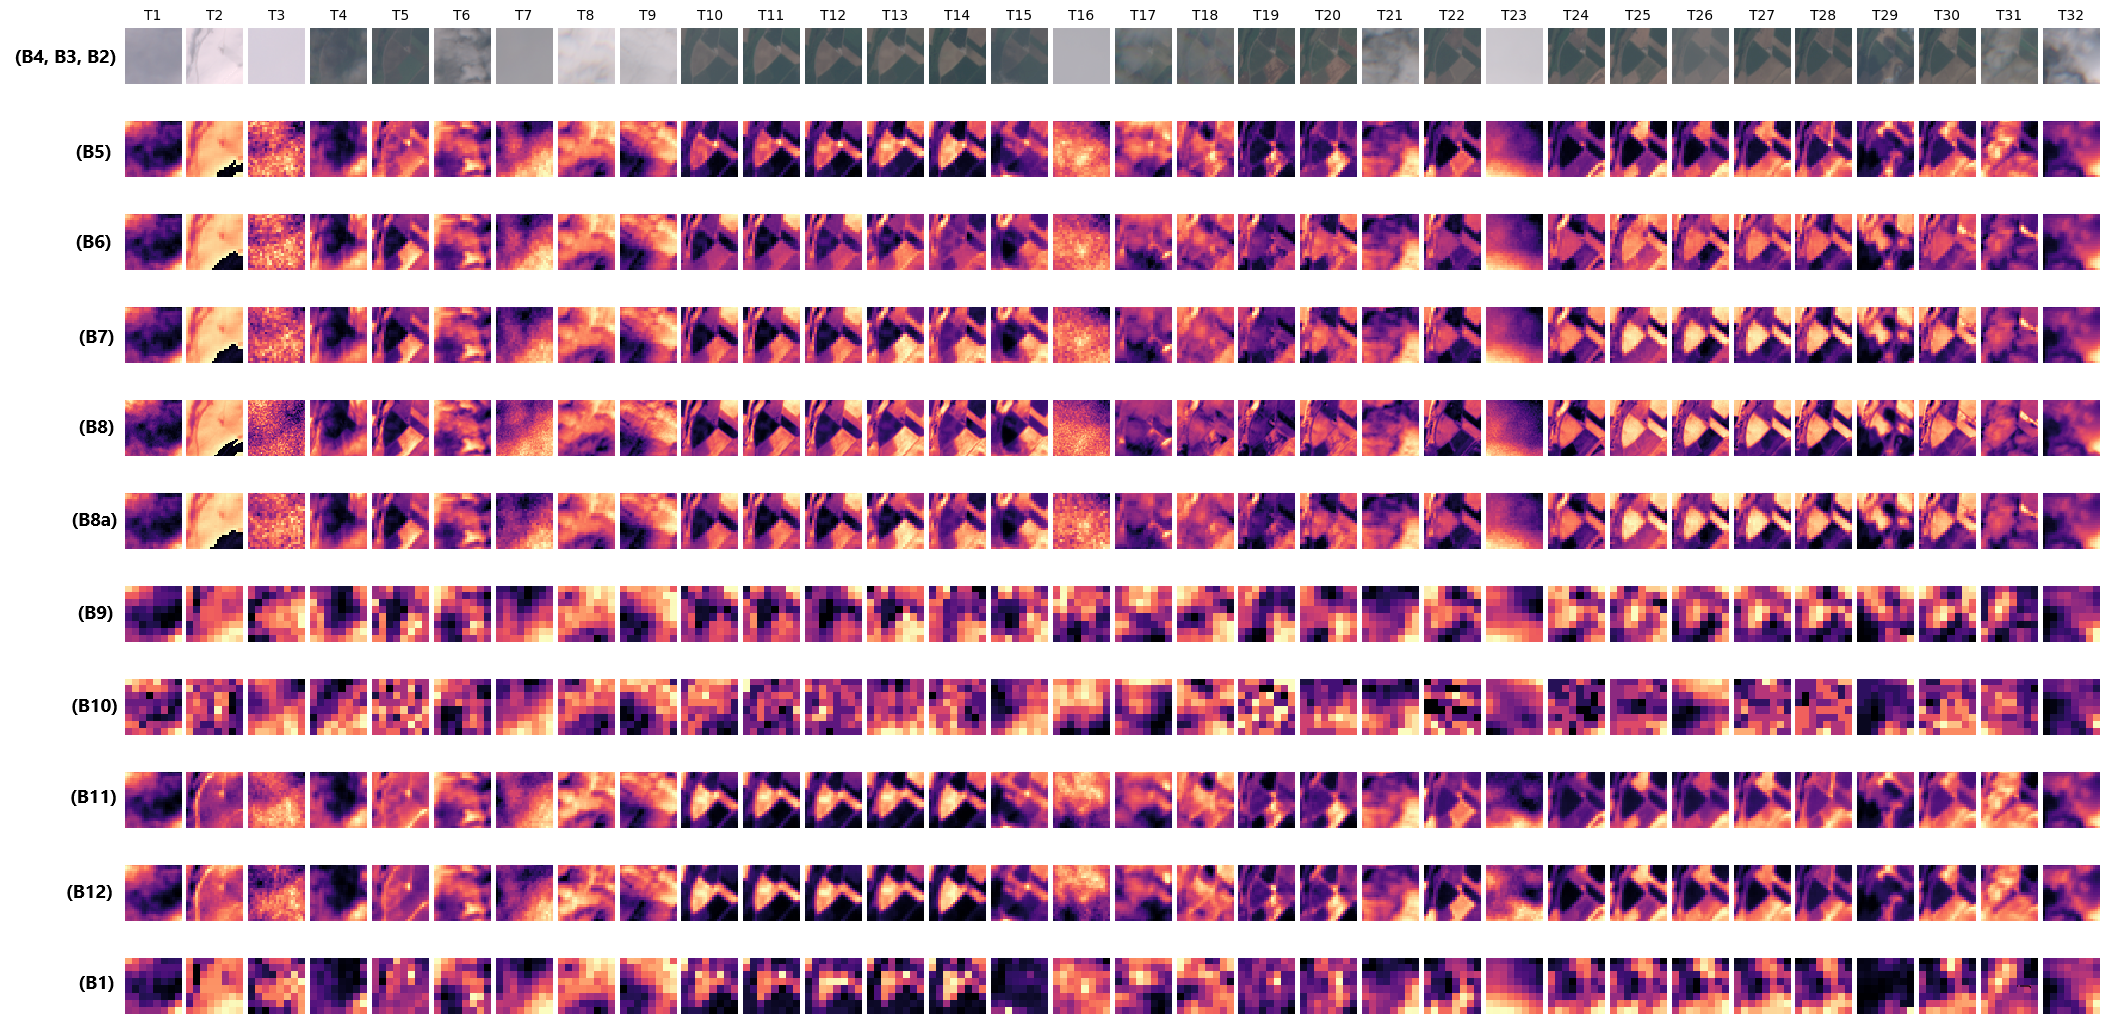
\includegraphics[width=1.05\textwidth]{Immagini/sperimentazione/INPUT_Ignore_Edit.png}
    \caption{Esempio di sequenza temporale fornita alla rete. Le colonne rappresentano le 
    immagini della sequenza, mentre le righe corrispondono alle diverse bande. In alto è 
    riportato il numero dell'immagine all'interno della sequenza, mentre a lato sono 
    indicate le bande (o la banda) rappresentate da ciascuna riga.}
    \label{fig:Ignore_INPUT}
\end{figure}


\begin{figure}[H]
    \centering
    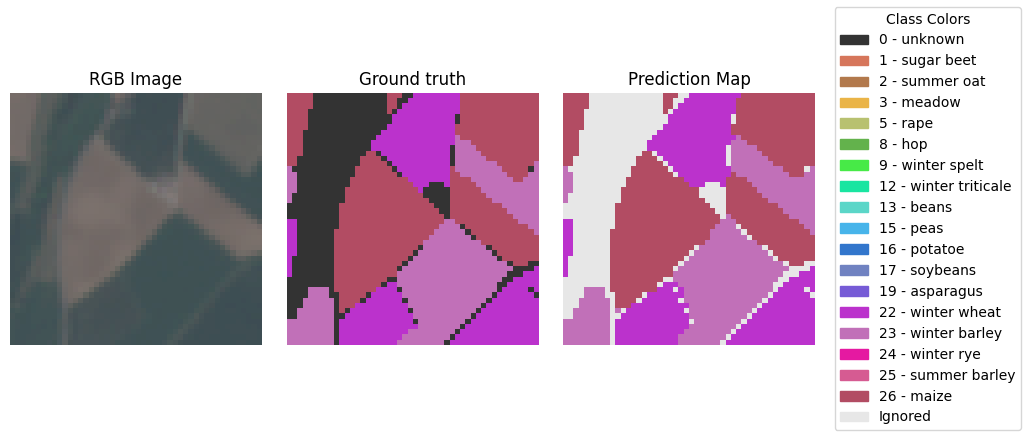
\includegraphics[width=1\textwidth]{Immagini/sperimentazione/LABEL_Ignore_Edit.png}
    \caption{Rappresentazione dell'input fornito alla rete, del risultato atteso e del risultato ottenuto.}
    \label{fig:Ignore_LABELS}
\end{figure}

Nella mappa di predizione della figura \ref{fig:Ignore_LABELS}, le aree in cui, 
nella mappa di verità, è presente la classe 0, sono state ignorate, in quanto non ci 
interessano le predizioni fatte dal modello in quei punti. Per quanto riguarda 
le predizioni fatte dal modello sulle aree interessate, queste risultano essere 
pressoché identiche alla mappa di verità.
Nella figura \ref{fig:Activations} sono riportate tutte le attivazioni 
delle diverse classi per l'esempio mostrato nella figura \ref{fig:Ignore_INPUT}.

\begin{figure}[H]
    \centering
    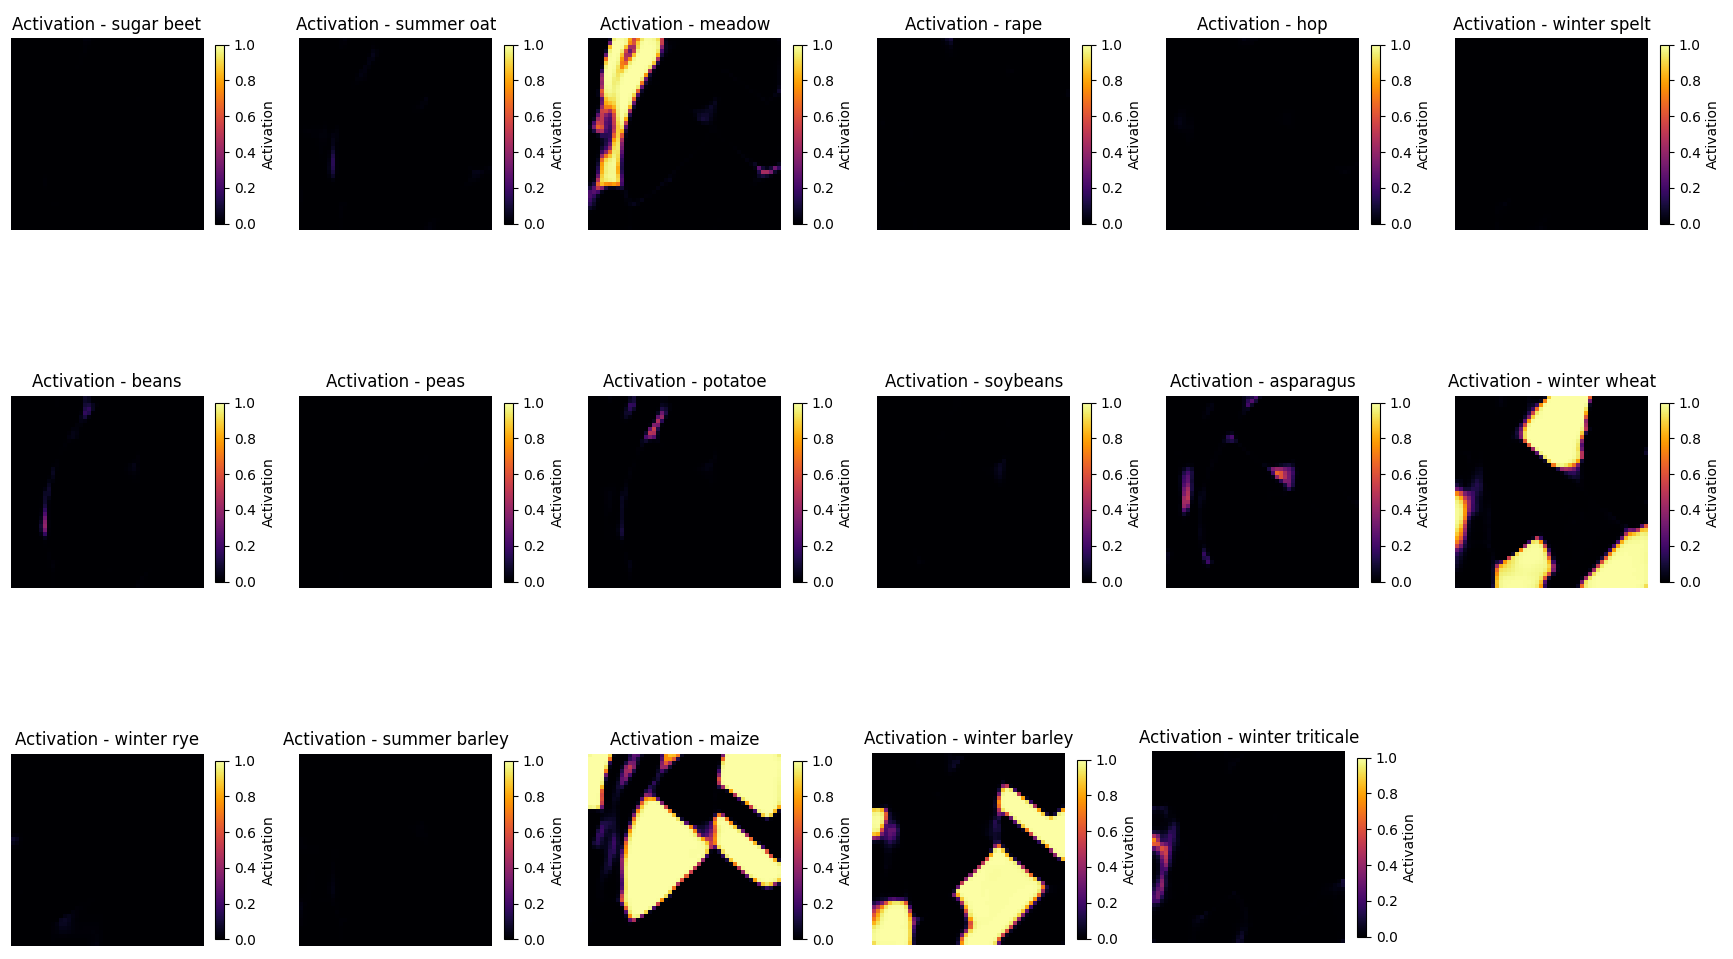
\includegraphics[width=1.05\textwidth]{Immagini/sperimentazione/ACTIVATIONS_Ignore_Edit_v2.png}
    \caption{Rappresentazione delle attivazioni di ogni classe.}
    \label{fig:Activations}
\end{figure}

Una cosa che spicca dalla figura \ref{fig:Activations} è come l'attivazione per la classe 
"\textit{meadow}" sia molto attiva nelle zone in cui, nella mappa di verità della figura 
\ref{fig:Ignore_LABELS}, è presente la classe "\textit{unknown}". Infatti, osservando 
l'immagine a colori della figura \ref{fig:Ignore_LABELS}, si potrebbe pensare 
che effettivamente ci sia un prato (\textit{meadow}).

\newpage
\subsection{Mosaicatura}
La mosaicatura è una tecnica utilizzata per ricostruire un'immagine di 
un'ampia area geografica a partire da tile elaborati singolarmente.
Essa consiste nell'unire in modo coerente i risultati delle predizioni effettuate su 
ciascun tile, preservando la continuità spaziale dell'immagine o dei dati.
Questo processo consente anche di capire se esiste continuità nelle 
predizioni del modello tra i diversi tile.
Le immagini qui sotto rappresentano un esempio di mosaicatura su alcuni blocchi 
di tile presi dal dataset di valutazione. A sinistra è riportata l'immagine a colori, mentre a 
destra le predizioni fatte dal modello.

\begin{multicols}{2}
{
    \begin{figure}[H]
        \centering
        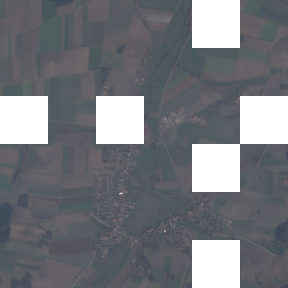
\includegraphics[width=0.38\textwidth]{Immagini/sperimentazione/MOSAICATURA_1_RGB.png}
        \caption{Mosaicatura a colori di un blocco di tile preso dal dataset di valutazione.}
        \label{fig:MOSAIC_RGB_1}
    \end{figure}
}
{
    \begin{figure}[H]
        \centering
        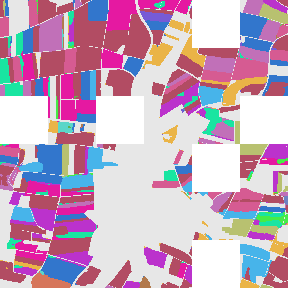
\includegraphics[width=0.38\textwidth]{Immagini/sperimentazione/MOSAICATURA_1_MASK.png}
        \caption{Mosaicatura delle predizioni dell'immagine \ref{fig:MOSAIC_RGB_1}.}
    \end{figure}
}
\end{multicols}

\begin{multicols}{2}
{
    \begin{figure}[H]
        \centering
        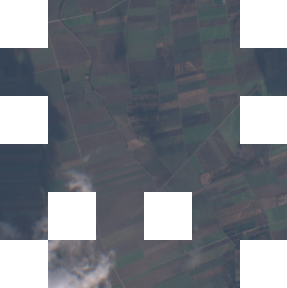
\includegraphics[width=0.38\textwidth]{Immagini/sperimentazione/MOSAICATURA_2_RGB.png}
        \caption{Mosaicatura a colori di un blocco di tile preso dal dataset 
        di valutazione.}
        \label{fig:MOSAIC_RGB_2}
    \end{figure}
}
{
    \begin{figure}[H]
        \centering
        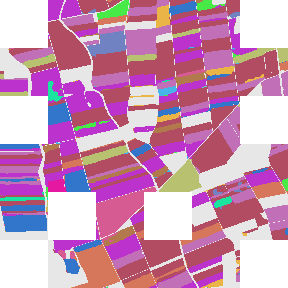
\includegraphics[width=0.38\textwidth]{Immagini/sperimentazione/MOSAICATURA_2_MASK.png}
        \caption{Mosaicatura delle predizioni dell'immagine \ref{fig:MOSAIC_RGB_2}.}
    \end{figure}
}
\end{multicols}
\newpage
\begin{multicols}{2}
{
    \begin{figure}[H]
        \centering
        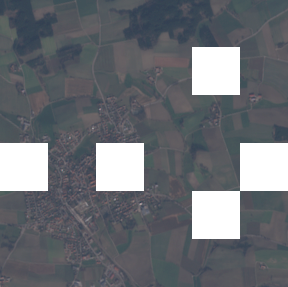
\includegraphics[width=0.36\textwidth]{Immagini/sperimentazione/MOSAICATURA_3_RGB.png}
        \caption{Mosaicatura a colori di un blocco di tile preso dal dataset di valutazione.}
        \label{fig:MOSAIC_RGB_3}
    \end{figure}
}
{
    \begin{figure}[H]
        \centering
        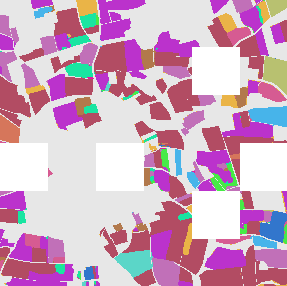
\includegraphics[width=0.36\textwidth]{Immagini/sperimentazione/MOSAICATURA_3_MASK.png}
        \caption{Mosaicatura delle predizioni dell'immagine \ref{fig:MOSAIC_RGB_3}.}
    \end{figure}
}
\end{multicols}
Come si può osservare dalle figure precedenti, il modello riesce anche ad avere una coerenza 
nelle predizioni tra tile differenti.
Se provassimo anche a considerare le aree dove nella mappa di verità si ha la classe è 0 
("\textit{unknown}"), la mosaicatura apparirebbe così:
\begin{multicols}{2}
{
    \begin{figure}[H]
        \centering
        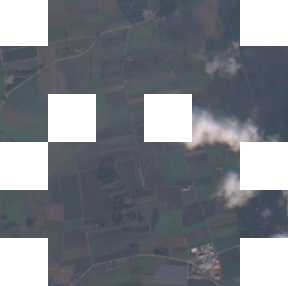
\includegraphics[width=0.36\textwidth]{Immagini/sperimentazione/ESEMPIO_MOSICATURA_2_INPUT_1.png}
        \caption{Mosaicatura a colori di un blocco di tile preso dal dataset di valutazione.}
        \label{fig:MOSAIC_RGB_4}
    \end{figure}
}
{
    \begin{figure}[H]
        \centering
        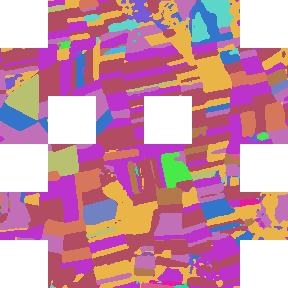
\includegraphics[width=0.36\textwidth]{Immagini/sperimentazione/ESEMPIO_MOSICATURA_2_PRED_1.png}
        \caption{Mosaicatura delle predizioni dell'immagine \ref{fig:MOSAIC_RGB_4}.}
    \end{figure}
}
\end{multicols}

\begin{multicols}{2}
{
    \begin{figure}[H]
        \centering
        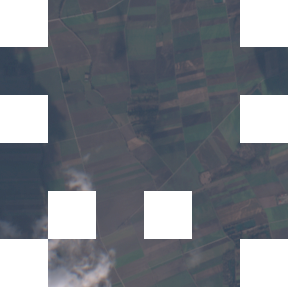
\includegraphics[width=0.36\textwidth]{Immagini/sperimentazione/ESEMPIO_MOSICATURA_2_INPUT_2.png}
        \caption{Mosaicatura a colori di un blocco di tile preso dal dataset di valutazione.}
        \label{fig:MOSAIC_RGB_5}
    \end{figure}
}
{
    \begin{figure}[H]
        \centering
        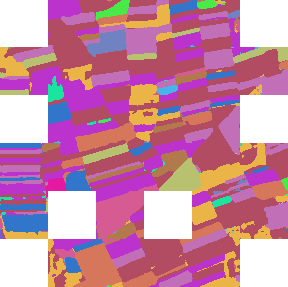
\includegraphics[width=0.36\textwidth]{Immagini/sperimentazione/ESEMPIO_MOSICATURA_2_PRED_2.png}
        \caption{Mosaicatura delle predizioni dell'immagine \ref{fig:MOSAIC_RGB_5}.}
    \end{figure}
}
\end{multicols}
